\chapter{Early Modern English (1500--1700)}\label{EModE}

\section{History and context}\label{EModE-history}

If you're reading this book, you have some competence in English. At the beginning of this chapter, take a moment to think about why that is the case. What does English mean to you? Why and how did you learn it?

Those of you who consider yourselves native speakers of English probably didn't grow up in England. At least, there are around four hundred million speakers of English in the world \citep{Crystal2006}, and the population of England is only a small fraction of that, so statistically it's unlikely. You've probably had occasion to consider how and why the English language got to where you are.

Those of you who consider yourselves non-native speakers will, presumably, have learned that language for a reason. Some people learn languages for the sheer fun of it, but more often there's some external motivation. In the case of English, perhaps it's because it's useful for trade, or for international communication, or for science,\is{scientific language} or so that you can access English-language books, games, films, websites, or TV shows. You've probably had occasion to consider how and why the English language came to be so dominant in these domains.

The events of the Early Modern English period are crucial for answering these questions. In 1500, English was spoken almost exclusively in England and Wales (and crucially to a rather limited extent in the latter) -- it was a language like any other, with no special \glossterm{gl-prestige}{prestige}\is{prestige} or status, and no worldwide reach. By 1700, English was well on the way to having the status it has today. In this chapter we'll see how that happened. But it's not English \textit{per se} that enjoys tremendous worldwide prestige\is{prestige} -- rather, it's a specific, fairly narrow set of varieties of English. How these standard varieties came to gain this status -- the process of \glossterm{gl-standardization}{standardization}\is{standardization} and the accompanying standard language ideology\is{standard language ideology} -- will be the guiding theme of this chapter.

\subsection{Standardization}\label{EModE-standardization}\is{standardization|(}
Academic linguists disagree about a great many things. One thing they agree on, however, is that it's meaningless to talk about one language being better or worse than another, at least in any objective linguistic sense. And yet among the general English-speaking public this attitude abounds. We all know someone who takes great pleasure in ``correcting'' the ``bad'' grammar of others (where by grammar they usually mean punctuation), or who delights in judging and shaming others based on their ``accent''. Even people who don't actively correct others believe very often that there is, when it comes down to it, a right or wrong way to use English.\footnote{And although M\'{i}\v{s}a is a sociolinguist,\is{sociolinguistics} she often asks herself when she's going to stop making certain non-native ``mistakes'' she catches herself making every now and then. But these ``mistakes'' could \textit{also} be approached from the angle of identity features with a range of social functions. The idea of ``correct'' vs. ``wrong'' is very deeply entrenched in our minds indeed!} We've talked about these prescriptive attitudes in detail in \chapref{LModE}. The ideal, for these people, is some sort of ``perfect'', ``accentless'' English as laid down by the great authorities. But what is this variety, and who speaks it? And can any variety truly be said to be ``accentless''?

People who think like this are in the grip of what \citet[67]{Lippi2012} terms \textsc{standard language ideology}:\is{standard language ideology}

\begin{quote}
a bias toward an abstracted, idealized, homogenous spoken language which is imposed and maintained by dominant bloc institutions and which names as its model the written language, but which is drawn primarily from the spoken language of the upper middle class.
\end{quote}

\noindent In this sense a standard is more of an abstract entity than an actually spoken (or even written) linguistic variety — though individual varieties may be perceived as closer to, or further from, the abstract standard ideal. The stranglehold of standard language ideology\is{standard language ideology} is strong, and it's probably fair to say that none of us are completely immune to it.\footnote{Or \textit{none of us \textbf{is}}, as particularly incurable prescriptivists\is{prescriptivism} will insist.} This is not the place for a full discussion of how it's maintained today or its pernicious consequences in society (see \citealp{Lippi2012} for an excellent discussion of these issues in the US context). But it's important to note that there's nothing universal about this ideology\is{standard language ideology} or the particular standard varieties associated with it. In fact, the Early Modern period played a crucial role in the standardization process, not only for English but for several European languages associated with emerging European world powers.

How, then, does a standard variety emerge? Norwegian sociolinguist\is{sociolinguistics} Einar Haugen's model, though fifty years old now, is still a widely accepted theory of standardization.\footnote{See \citet{JosephVostersRutten2020} for a critical assessment of Haugen's model after fifty years of research and reflection on its enduring influence.} Haugen observes that standard varieties are inextricably bound up with nations and the rise of nation-states\is{nation-states}:

\begin{quote}
The invention of printing,\is{printing press} the rise of industry,\is{industrial revolution} and the spread of popular education have brought into being the modern nation-state, which extends some of the loyalties of the family and the neighborhood or the clan to the whole state. Nation\is{nation-states} and language have become inextricably intertwined. Every self-respecting nation has to have a language. Not just a medium of communication ... but a fully developed language. Anything less marks it as underdeveloped. \citeyearpar[927]{Haugen1966}
\end{quote}

\noindent Haugen is in agreement with many modern historians (e.g. \citealp{Foucault2007,Hobsbawm1990}) that developments in the sixteenth and seventeenth centuries were crucial in leading to the nation-state\is{nation-states} as the main unit of political organization on the world stage. Since language is a central part of identity, and it was in the nation-state's interest to foster a shared identity, ``one nation,\is{nation-states} one language'' policies and pressures (see \citealp{Piller2015}) have historically been an important driving force of standardization. Haugen also outlines a four-step model of how the standardization process unfolds, schematized in Figure \ref{fig:standardization}. The four steps -- better thought of as overlapping subprocesses -- are \textsc{selection}, \textsc{elaboration}, \textsc{codification} and \textsc{acceptance}.

\begin{figure}
          \begin{tikzpicture}
      \filldraw[fill=lsLightGreen,draw=black] (0,0) rectangle (4,2);
      \node[align=center] at (2,1) {\textbf{Codification}\\of forms\\c. 1600--1800};
      \filldraw[fill=lsLightWine,draw=black] (4,0) rectangle (8,2);
      \node[align=center] at (6,1) {\textbf{Elaboration}\\of functions\\c. 1500--1800};
      \filldraw[fill=lsMidBlue,draw=black] (0,2) rectangle (4,4);
      \node[align=center] at (2,3) {\textbf{Selection}\\of norms\\c. 1400--1600};
      \filldraw[fill=lsYellow,draw=black] (4,2) rectangle (8,4);
      \node[align=center] at (6,3) {\textbf{Acceptance}\\by community\\c. 1500--now};
      \node[rotate=90] at (-0.2,1) {language};
      \node[rotate=90] at (-0.2,3) {society};
      \node at (2,4.2) {form};
      \node at (6,4.2) {function};
     \end{tikzpicture}
     \caption{Standardization according to \citet[933]{Haugen1966}. Dates for English are approximate, and are our interpretation.}
     \label{fig:standardization}
\end{figure}

\largerpage
\noindent \textsc{Selection} gets to the heart of the question: whose variety becomes the basis for the new standard? Standards, like the nation-states\is{nation-states} they belong to, are supposed to be stable and unified, so variation is ruled out, and a single ``correct'' form needs to emerge. William Caxton,\ia{Caxton, William} who introduced the printing press\is{printing press} into England in 1476, was well aware that he needed to make choices at all linguistic levels, not only spelling\is{orthography} (see the next section, \sectref{EModE-GVS}) and the lexicon (e.g. \textit{egges} vs. \textit{eyren} `eggs'; see the text in \sectref{ME-Caxton}), but also morphology, and syntax.\footnote{For more discussion of the printing press itself and the physical process of printing, see \citet[159--162]{vanGelderen2014}.} The choices made by Caxton and other printers\is{printing press} at the end of the Middle English period and the start of the Early Modern period were certainly influential in selecting variants that would become part of the emerging standard, because they permitted documents to be circulated on a much larger scale than ever before. At the same time, it's important not to overstate the role of printing in standardization. For one thing, it wasn't an accident that the printing presses were based in London, which even then was the political and economic centre of England. They were also just around the corner from the Chancery,\is{Chancery} the centre of royal document production, which had to a certain extent established its own norms during the fifteenth century \citep{Fisher1977}, at least for spelling\is{orthography} -- and it is clear that these Chancery\is{Chancery} norms affected the variety adopted by the printers.\is{printing press}

A common narrative in history of the English language textbooks is based on \citet{Samuels1963} and \citet{Fisher1977}, and goes like this: migrating\is{migration} merchants from the East and Central Midlands of England brought their English with them to London, and this became the basis for the standard. This is at best an oversimplification. London was certainly a centre of immigration during the period, but from all areas of the country, in particular the southern counties surrounding the city.\footnote{These processes of migration\is{migration} may have been a crucial factor in determining the course of the Great Vowel Shift:\is{vowels}\is{Great Vowel Shift} see \sectref{EModE-GVS}!} Not all of the features that eventually make it into Standard English have their origin in the East Midlands, and not all of the spelling\is{orthography} features found by \citet{Fisher1977} in Chancery\is{Chancery} texts make it into Standard English either: see \citet{Wright1996}, the papers in \citet{Wright2000}, and \citet{Benskin2004}. Much still remains to be understood about the process of selection, but we can at least say with confidence that it was not a single variety that was ``selected'': instead, selection seems to have operated opportunistically, with individual linguistic features finding their origin in Northern, Southern and Midlands varieties,\is{regional variation} Chancery\is{Chancery} spelling\is{orthography} norms, literary texts, the spoken and written usage of merchants, and beyond. Standard English is a mongrel, not a purebred. And research in this area continues! See \citet{AuerGordonOlson2016} for discussion of a recent project that aims to shed more light on this issue.

\textsc{Elaboration} involves the spread of a variety to domains that had previously been dominated by other languages: for instance, law,\is{legal language} science,\is{scientific language} medicine, politics, religion, philosophy, and the like. The ``one nation,\is{nation-states} one language'' ideology demands that a standard language should be usable for any purpose. But in order to function well in these new domains, new lexical items need to be created. These come from the usual sources: either lexical borrowing,\is{borrowings} or word formation\is{word formation} via \glossterm{gl-derivation}{derivation} or \glossterm{gl-compounding}{compounding}. The linguistic process and consequences of elaboration are discussed in \sectref{EModE-lexicon}, on the Early Modern English lexicon.

\hspace*{-5pt}One important domain in which the English language was breaking new ground during the Early Modern English period is that of religion.\is{Christianity} In the early sixteenth century, in what is now Germany, Martin Luther\ia{Luther, Martin} was influentially propounding the view that Christianity\is{Christianity} needed to return to its roots in scripture, dispensing with many of the traditions of the Catholic church. This new perspective -- Protestantism -- spread like wildfire across Europe, and was adopted by the English King Henry VIII\ia{Tudor, Henry (King Henry VIII)} in the 1530s. Its linguistic importance lies in the fact that Luther and the other reformers were insistent that the clergy use modern European languages to communicate with the people rather than \ili{Latin}. Luther himself translated the Bible into \ili{German} from \ili{Hebrew} and \ili{Greek}. Before the Reformation, translating the Bible into English was illegal: William Tyndale\ia{Tyndale, William} produced a partial translation, but was convicted of heresy, sentenced to death by strangulation, and finally burned at the stake in 1536. Myles Coverdale\ia{Coverdale, Miles} and John Rogers\ia{Rogers, John} completed the task, however, and their version became widely circulated, with an important influence on other major translations such as the famous King James\ia{Stuart, James (King James I)} Bible of 1611.\is{Christianity}

Natural philosophy (the origin of what we now call ``science'')\is{scientific language} also saw an increase in English-language texts, especially during the seventeenth century. Robert Boyle's\ia{Boyle, Robert} \textit{Sceptical Chymist} (published in 1661) was a seminal work in chemistry. Isaac Newton\ia{Newton, Isaac} published his most famous work, \textit{Philosophiæ Naturalis Principia Mathematica}, in \ili{Latin} in 1687, but his second major book \textit{Opticks} (1704), on the nature of light, was published in English.\is{scientific language}

If the goal of elaboration can be described as ``maximal variation in function'', the goal of \textsc{codification} is ``minimal variation in form'' \citep[931]{Haugen1966}. In \chapref{LModE} we've already seen how codification takes shape in the history of English: \sectref{prescriptivism} mentions the grammars, dictionaries, and pronunciation and usage guides that proliferate during the seventeenth and eighteenth centuries in particular. Nowadays we tend to take the existence of such books for granted -- where else would you check how to use the ``correct'' form? -- but the fact is that many languages that have not undergone standardization do not have grammars or dictionaries written for them, and in the history of English there were no serious attempts to write books like these before the Early Modern period. We'll see an example of the effects of codification and the prescriptivism\is{prescriptivism} it gives rise to in \sectref{EModE-stranding}, on preposition stranding.\is{preposition stranding} It's also worth noting at this point that codification took different paths in Britain and North America: see the text by Noah Webster\ia{Webster, Noah} in \sectref{LModE-Webster} in the previous chapter for an early US perspective on standardization. \citet[chapter 4]{Millar2012} has a good discussion of codification in English.


\begin{miscbox}{An English Academy?}
Other countries went further than the United Kingdom and established an official institution with responsibility for the country's (standard) language. The \textit{Accademia della Crusca} was founded in 1583 in Florence, and is the world's oldest linguistic academy. The powerful \textit{Académie française} followed in 1635 in France. In the seventeenth and early eighteenth centuries there were calls to set up a similar institution: in 1665 a group including John Dryden\ia{Dryden, John} (see \sectref{EModE-stranding}) actually met at Gray's Inn in London to plan an academy, but their efforts came to nought. The most famous such suggestion came from the political writer and satirist Jonathan Swift,\ia{Swift, Jonathan} in his 1712 \textit{Proposal for Correcting, Improving and Ascertaining the English Tongue}. This proposal briefly won royal support from Queen Anne,\ia{Stuart, Anne (Queen Anne)} but was nevertheless ultimately unsuccessful: Anne died in 1714, and subsequent monarchs did not return to the idea. See \citet[236--238]{MillHay2018} for more.
\end{miscbox}


\noindent Finally, ``a standard language, if it is not to be dismissed as dead, must have a body of users'' \citep[933]{Haugen1966}. The gradual orientation of a speech community towards a single abstract standard is the process of \textsc{acceptance}. Far from being an active, deliberate process, what Haugen describes as acceptance is driven by a mixture of carrot and stick. On the one hand, users of the standard have access to greater power and more influential positions, and a potent signifier of (national)\is{nation-states} group identity.\footnote{Which also, of course, plays a central role in \textit{constituting} that group identity.} On the other hand, those who cannot use the standard, or choose not to, have reduced access to those opportunities, and will often face overt scorn and prejudice. Thus, a complex web of conscious and subconscious incentives keeps the ideal of a standard language enmeshed in people's minds. In this respect, very little has changed over the past centuries: once again, see \citet{Lippi2012} on the toxic present-day effects of standard language ideology.\is{standard language ideology}

Throughout this chapter we'll come back to standardization and its effects, which are felt at all linguistic levels.

\subsection{The Empire strikes}\label{EModE-colonial}\is{colonialism|(}\is{British Empire|(}

By itself, the standardization\is{standardization|)} process doesn't explain how English came to be a world language. For that, we need a little history of empire.

At the beginning of the Early Modern period, England (with Wales), Scotland, and Ireland were separate countries. The three kingdoms came to share a single ruler when James VI\ia{Stuart, James (King James I)} of Scotland acceded to the thrones of England and Ireland in 1603, though they were not formally unified as a single ``United Kingdom'' until 1707. On the world stage, however, England in particular was flexing its military and political muscles throughout the period. The ``discovery'' of the Americas by Columbus\ia{Columbus, Christopher} in 1492 had opened the door for an international scramble to snap up as much territory and as many resources as possible on this ``new'' landmass, and elsewhere too; France, the Netherlands, Portugal, and Spain were other important European actors. The fact that the territories being snapped up were already occupied by other humans who had been there much longer didn't stop colonies from being established around the world. Jamestown, the first colony in what is now the United States of America, was established in 1607, and Plymouth, Massachusetts, the first permanent colony, in 1620. The Massachusetts Bay Colony was founded in 1629, and the well-known Harvard University emerged here in 1636.

Any good history book will tell you about the rise of the United States, and the linguistic aspects of this rise have already been discussed in \sectref{LModE-AmE} in the previous chapter. It's useful to know that many of the colonists who made the long journey across the Atlantic did so for religious reasons:\is{Christianity} the founders of Plymouth -- the famous Pilgrim Fathers who sailed aboard the \textit{Mayflower} -- were Protestants, Puritan separatists who wanted to live apart from the Church of England, and the founders of the Massachusetts Bay colony were Puritans who wanted to reform the Church. The Jesuits -- an evangelizing Catholic society heavily involved in the Counter-Reformation -- also did their bit to spread English to the Americas and the rest of the world. Jesuits set up missions all over the world, with educational goals that included teaching European languages to colonized peoples. The Province of Maryland was founded in 1632 as a haven for Catholics, and the Jesuits there played an important role in establishing relations between colonizers and Native Americans -- attempting to teach the latter English and convert them to Christianity,\is{Christianity} while also carrying out some of the earliest translations of religious texts into the \ili{Algonquian} languages.


\begin{peoplebox}{Two queens}

\begin{figure}[H]
%     \subfigure[~]{ \label{fig:MaryStuart}
            \includegraphics[height=.33\textheight]{chapters/img/Mary_Stuart_Queen.jpg}
%             }
~~~~
%     \subfigure[~]{ \label{fig:ElizabethTudor}
        \includegraphics[height=.33\textheight]{chapters/img/Elizabeth1England.jpg}
%         }
    \caption{Mary Stuart and Elizabeth Tudor}
\end{figure}

Throughout the Early Modern period, Britain was dominated by two rapacious dynasties, the Tudors and the Stuarts. During the second half of the sixteenth century, two powerful women ruled England and Scotland: Elizabeth Tudor (Elizabeth I of England)\ia{Tudor, Elizabeth (Queen Elizabeth I)} and Mary Stuart (``Mary, Queen of Scots'').\ia{Stuart, Mary (Queen of Scots)} Mary, a Catholic, was forced to abdicate, and spent eighteen years in captivity before eventually being executed: see \citet{Guy2004} for a scholarly but lively account.

% \begin{wrapfigure}{l}{0.2\textwidth}
%     \caption{Mary Stuart.}
%
% \end{wrapfigure}

The two women are linguistically very interesting. Mary Stuart grew up in France, and was natively bilingual\is{multilingualism} in \ili{French} and \ili{Scots}, as well as able to write in English, \ili{Italian} and \ili{Latin}. Her letters are a linguistic treasure trove. As for Elizabeth, she was described posthumously as having spoken nine languages, including \ili{Cornish}, \ili{Irish} and \ili{Welsh}, at near-native level -- though we probably shouldn't take this glowing testimony at face value. We know, however, that throughout her life she translated \ili{Latin} and \ili{Greek} works: in 2019, a manuscript\is{manuscripts} of a translation of Tacitus was shown to be written by her \citep{Philo2020}.

\end{peoplebox}


\noindent English colonizers also reached India, the Caribbean, and Africa during the Early Modern period. The African situation was particularly important for the ongoing developments in the United States, since this continent furnished the seaborne Europeans with an almost inexhaustible supply of people to be enslaved.\is{slavery} As peoples, plants, products, diseases and ideas were taken from continent to continent -- called the \textsc{Columbian Exchange}\is{Columbian Exchange} after Christopher Columbus\ia{Columbus, Christopher} \citep{Crosby1972} -- the world changed irrevocably. Diseases such as smallpox (from Europe) and yellow fever (from West Africa) are estimated to have killed 80--95\% of the Native American population (\citealp[167]{Newson2001} and references cited there; \citealp[165]{NunnQian2010}). Subsequently, the circulation of different forms of crops and livestock allowed for major population increases in all of these countries: tomatoes, potatoes and maize were all brought back to Europe from the Americas (see \sectref{EModE-lexicon} for the origins of words like these!), and farm animals such as cows, horses and chickens were transported to the Americas from Europe, for instance. The most obvious linguistic impact of the Columbian Exchange\is{Columbian Exchange} was the spread of English (alongside other languages of Europe such as \ili{Spanish} and \ili{Portuguese}), but of course English itself was dramatically changed by these events too, through lexical innovations and the emergence of new varieties shaped by language contact around the globe.\is{globalization}\is{colonialism|)}\is{British Empire|)}

In what follows, you'll learn about some of the main linguistic changes characteristic of this period.

\section{Sounds}
\largerpage
In this section, you are going to learn about what is considered one of the most important sound changes in the history of the English language: the Great Vowel Shift\is{Great Vowel Shift} (sometimes abbreviated to GVS).\is{vowels} However, the fact that we only focus on this sound change in the Early Modern English period should not leave you thinking that this is the only interesting aspect of Early Modern English phonology. Because the Great Vowel Shift\is{vowels} is a fairly complex phenomenon (as you will soon find out for yourself), for practical reasons we will not cover all the other exciting phonological and phonetic aspects of Early Modern English, such as the loss of certain consonants\is{consonants} (postvocalic /h/;\is{/h/-dropping} some cases of /t/, as in \textit{castle} /kɑːsɫ/; some cases of /l/, as in \textit{talk} /toːk/ and \textit{walk} /woːk/); changes related to unstressed vowels;\is{vowels} changes in the quality of the vowels in words like TRAP and DRESS;\is{vowels} the change from /aʊ/ to /ɔː/, as in \textit{cause} [kauz] > [kɔːz]; and certain diphthong\is{merger} mergers.\footnote{Check out \citet[248--255]{MillHay2018} and \citet[Chapter 9]{Nevalainen2006} if you're hungry for more on these.}

\subsection{The Great Vowel Shift}\label{EModE-GVS}
\subsubsection{What is the Great Vowel Shift?}\is{vowels|(}\is{chain shifts|(}\is{Great Vowel Shift|(}
Early Modern English is full of variation, and long vowels are particularly interesting. They show variation related to vowel quality, and some also show variation in whether or not this quality changes from the beginning to the end of a vowel, i.e. whether they are monophthongs or diphthongs. Such variation in long vowels is primarily due to the Great Vowel Shift. The Great Vowel Shift presents us with a rather grand vowel change, as it affected the \textit{entire} system of long monophthongs of the language. As long as you were a long monophthong, your quality eventually changed. Some of the variants were those we are familiar with from standard Present Day English. However, other variants no longer survive in standard Present Day English -- these are the historically older variants. We can see the older variants in Figure \ref{fig:EModEVowels}, which shows you the very early Early Modern English long monophthongs.

\begin{figure}
        \includegraphics[height=.25\textheight]{chapters/img/EModEVowelsa.pdf}
    \caption{Early Modern English long monophthongal vowel system}
    \label{fig:EModEVowels}
\end{figure}

\noindent You will notice the following. First, the words you will recognize from Present Day English contained vowel qualities that differ from those they have in Present Day English -- these are the pre-shift vowel qualities. Second, there seems to be a fairly neat correspondence between the vowel qualities implied by the IPA symbols and the graphemes (letters). Thus, the word \textit{bite} is spelt with an <i> and pronounced with an [i] as well. You may be a bit puzzled about \textit{mouth}, which was pronounced as /mu:θ/ and spelt with an <ou> rather than an <u>. However, as we will see in the next chapter (\sectref{ME-graphical}), <ou> and <u> both reflected [u] at the time. You will also notice that there are two types of e and two types of o, corresponding to [e] and [ɛ], and [o] and [ɔ], respectively. One thing not visible from the figure is that these long monophthongs have corresponding short monophthongs, i.e. corresponding in vowel quality, but differing in vowel quantity (i.e. duration, whether the vowel is long or short).

Now that we have established what the pre-shift long monophthongal system was like, you are probably burning to find out just what exactly happened to get us to the vowel qualities we are used to for the words in Figure \ref{fig:EModEVowels} in standard Present Day English. As indicated in Figure \ref{fig:EModEVowels2}, the vast majority of the vowels have changed in quality by being raised. Thus, the vowel in \textit{boat} [bɔːt] was raised to [boːt], and later also became a diphthong ([boʊt], [bəʊt]),\is{diphthongization} although there are still dialects of English that preserve the monophthongal quality, as we will see below. Similarly, the vowel in \textit{boot} was also raised, although this time the higher quality is that of [u], giving us [buːt]. This is a nice example of a shift: a change in the phonetic realization of one vowel \glossterm{gl-phoneme}{phoneme} is connected to a change in the realization of another vowel phoneme. Importantly, the vowel phoneme in words like \textit{boat} did not become the same as that found in words like \textit{boot} -- speakers today still produce and perceive these as two distinct categories.\footnote{We saw the same process in \chapref{englishtoday} when the Northern Cities Shift\is{Northern Cities Shift} was introduced.} You may then wonder what happened to Early Modern English /uː/, considering this vowel has nowhere higher to go. What happened to /uː/ is diphthongization:\is{diphthongization} the vowel in \textit{mouth} [muːθ] ultimately became [maʊθ].

\begin{figure}
        \includegraphics[height=.25\textheight]{chapters/img/EModEVowels2a.pdf}
    \caption{The Great Vowel Shift in a nutshell -- vol. 1}
    \label{fig:EModEVowels2}
\end{figure}

The front vowels changed in a similar fashion, although they present us with some complications in contrast to the back vowels. As you would expect by now, the highest vowel, /iː/, diphthongized,\is{diphthongization} giving us a change from \textit{bite} [biːt] to (ultimately) [baɪt]. Also as you would expect, \textit{beet} [beːt] was raised to [biːt]. So far so good. But then we come across \textit{beat} [bɛːt]. Again as expected, the vowel in [bɛːt] was raised to [beːt], but this is not where the raising stopped. The raising continued, so that the original /ɛː/ vowels were raised to [iː], taking a stop on this journey at [eː]. And yes, if you were reading carefully, you may have come to this realization: the vowel phonemes in words such as \textit{beet} and \textit{beat} merged\is{merger} into a single category, into a single phoneme. This is no longer a phonetic change whereby one vowel quality changes into another vowel quality. What happened here is that one vowel phoneme was lost: we have a merger\is{merger} of the two.

We have not mentioned what happened to the vowel phoneme found in words such as \textit{name} yet. The vowel in \textit{name} [naːm] got raised, just like most of the other vowels, becoming [nɛːm] and ultimately diphthongizing into [nɛɪm]. The final diphthongization\is{diphthongization} change, however, did not take place in all dialects of English, and again, as we will see later on in this section, some dialects still have a monophthong in words like \textit{name}. Figure \ref{fig:EModEVowels3} sums these added observations up.

\begin{figure}
        \includegraphics[height=.25\textheight]{chapters/img/EModEVowels3a.pdf}
    \caption{The Great Vowel Shift in a nutshell -- vol. 2}
    \label{fig:EModEVowels3}
\end{figure}

\noindent Now that we have got the basics of the Great Vowel Shift off our shoulders, there is no time to relax, because things are just getting started. First of all, the raising phenomena and the diphthongization\is{diphthongization} steps were presented to you in a way that really simplified what took place during the shift. A change of this magnitude takes time, and the Great Vowel Shift took centuries: some would even argue that it may have never quite reached completion, at least in some dialects of English. First of all, there are some exceptions, irregularities,\is{irregularities} to the Great Vowel Shift. The vowels in words such as \textit{great}, \textit{steak}, \textit{yea}, and \textit{break} were not raised, and their original [ɛ] therefore merged\is{merger} with the vowel in the \textit{name} class, giving us homophones such as \textit{break} and \textit{brake}. Another unexpected outcome of the shift is the vowel qualities we get in words such as \textit{death} and \textit{head}, where the originally long vowel [ɛː] became a short [ɛ] \citep[251]{MillHay2018}. This serves as a good reminder: the Great Vowel Shift only affected \textit{long} monophthongs. If an originally long vowel became short before the Great Vowel Shift kicked in, it was unaffected by the shift. An interaction of various vowel shortening\is{vowel shortening} processes and the Great Vowel Shift has resulted in the ``irregular''\is{irregularities} vowel pairs in words such as \textit{sane} /s\textbf{ɛɪ}n/ and \textit{sanity} /s\textbf{a}nɪti/, to the chagrin of non-native English speakers; the spelling\is{orthography} nevertheless reflects the pre-GVS stage. A related outcome of the shift are seemingly illogical grapheme-phoneme correspondences, as in \textit{round} /raʊnd/ but \textit{soup} /suːp/, where <ou> corresponds to two different vowel phonemes. What happened here? What explains this inconsistency is the fact that \textit{round} was borrowed\is{borrowings} into English in time to be affected by the shift, whereas \textit{soup} wasn't, and hence the grapheme-phoneme discrepancy! There are more complexities, but we believe you have had quite enough of those at this point.


\begin{soundbox}{Hotly debated}
Some of the changes described above include intermediate stages. /iː/ and /uː/ in particular have been a popular subject of discussions about the GVS. To give a more specific example, one of the mainstream proposals is that the [iː] in \textit{night} [niːt] went through an [əɪ] stage before reaching today's standard [aɪ]. But the by far most passionate debate surrounding the shift concerns which vowel phonemes started changing first and when, and which changes therefore motivated other changes that happened. If you're particularly intrigued by any of these topics, we recommend \citet{McMahon2006} on the famous Stockwell\ia{Stockwell, Robert} \& Minkova\ia{Minkova, Donka} vs. Lass\ia{Lass, Roger} debates.  What is more, some researchers have even questioned whether all the different vowel changes involved are in fact a single event, whether the shift started already in Early Middle English, or actually even earlier, and which phenomena should or should not be subsumed under the label of the Great Vowel Shift (see e.g. \citealp[chapter 1]{Stenbrenden2016} and again \citealp{McMahon2006}).
\end{soundbox}


\subsubsection{Further outcomes of the Great Vowel Shift}
There are two important outcomes of the Great Vowel Shift which are useful to know for anyone engaging with Present Day English phonetic variation. As already mentioned, not all dialects of English have undergone all of the stages of the shift. Some dialects in the UK have monophthongs in words such as \textit{face} and \textit{name} (the FACE lexical set) in contrast to the standard diphthong, and also in words such as \textit{goat} and \textit{boat} (the GOAT lexical set). Similarly, in some dialects of English, the pre-shift /uː/ vowel did not diphthongize,\is{diphthongization} giving us Present Day English \textit{loud} [luːd], \textit{cow} [kuː], and \textit{mouth} [muːθ] (the MOUTH lexical set). Monophthongal variants of the vowels found in words such as FACE and GOAT are typical of northern English dialects, for instance. You will be asked to explore this regional variation\is{regional variation} in Exercise \ref{EModE-GVS-exercise}. 

In this context, it is worthwhile to also mention accents such as Indian English\il{English, Indian} and Welsh English\il{English, Welsh} in particular. These have features that at first sight look like traces of the pre-Great Vowel Shift state of affairs. Namely, one of the traditional features of Indian English is monophthongal pronunciations of the vowels we find in words such as GOAT and FACE: /goːt/ for /gəʊt/, and /feːs/ for /fɛɪs/ \citep[626]{Wells1982c}. The same goes for traditional Welsh English accents as well \citep[382--385]{Wells1982b}. This raises interesting questions. Could these represent an older historical stage of the phonological system of English? Regarding Welsh English,\il{English, Welsh} \citet[382--383]{Wells1982b} strongly implies that the monophthongal pronunciations are due to the influence of \ili{Welsh}, rather than a historical leftover of pre-GVS days. Furthermore, in \textit{some} South Wales English accents, two groups of words are attested where one group shows monophthongal pronunciations and the other diphthongal ones: \textit{toe} [toː] vs. \textit{tow} [tou $\sim$ tɔu], \textit{nose} [noːs] vs. \textit{knows} [nous $\sim$ nɔus].\footnote{Welsh English traditionally lacks the voiced alveolar fricative /z/.} \citet[384--385]{Wells1982b} proposes that all of these present older borrowings,\is{borrowings} whose production is most likely based on the spelling.\is{orthography} As non-native English speakers (who aren't necessarily widely exposed to native English), learners with near 1:1 grapheme-phoneme vowel correspondences in their L1, as is the case in Welsh, can easily think that if a word is spelt as a <nose>, the spelling\is{orthography} surely indicates something like an o (i.e. a monophthong). Regarding Indian English,\il{English, Indian} one could speculate that the presence of monophthongs could be put down to the vowel system of the native language(s) of the learners, or alternatively be a historical archaism (\citealp[626]{Wells1982c} for a tentative thought), or possibly a mixture of the two.

The second important outcome of the Great Vowel Shift is the discrepancy between the spelling\is{orthography|(} system of Present Day English and the actual pronunciation supposed to be reflected by this spelling system, as evidenced for instance by the presence of webpages titled ``Absolutely Ridiculous English Spelling'',\footnote{See here: \url{http://www.say-it-in-english.com/SpellHome.html}.} as well as by poems\is{poetry} composed to illustrate the ambiguity of the English spelling system, such as \emph{The Chaos} by Gerard Nolst Trenité.\ia{Nolst Trenité, Gerald} \citet[231]{MillHay2018} state that ``[t]he sixteenth century was perhaps the last time a thoroughgoing reform of English spelling was possible. Soon thereafter, the spread of printed\is{printing press} books was to make the vested interest in older customs too great to be overthrown [...].'' Some have blamed the Great Vowel Shift for the numerous discrepancies between the spelling and the pronunciation of the English language. It doesn't take too much online searching to come across claims such as ``A lot of English's ``crazy'' spelling can be explained by the Great Vowel Shift.''\footnote{\url{http://languagenerdadventures.blogspot.com/2009/06/great-vowel-shift.html}.} And here's the explanation provided: ``Because spelling was pretty much already established at the time the Great Vowel Shift occurred, the pronunciation changed while the spelling did not. And that is why English has such ``crazy'' spelling.'' But is this really a good enough explanation?

Irish playwright and social commentator George Bernard Shaw\ia{Shaw, George Bernard} was one of the individuals in support of a spelling reform during his times (1856--1950). To illustrate the need of a spelling reform, Shaw referred to one of the rather absurd examples invented to demonstrate the idiosyncracies of the English spelling: the word \textit{fish} might as well be spelt as <ghoti>. Why? 1. <gh> is not used just to signal /g/ (\textit{\textbf{gh}ost}) but also /f/ (\textit{tou\textbf{gh}}); 2. <o> corresponds to /ɪ/ in the word \textit{w\textbf{o}men}; 3. and <ti> corresponds to /ʃ/ in a number of words (e.g. \textit{pronuncia\textbf{ti}on}). As we can see from the <ghoti> example, it is certainly not just the vowels that present us with the lack of one-to-one spelling-pronunciation correspondence. This means that the ``crazy'' English spelling cannot really be blamed solely on the Great Vowel Shift.

There is another problem with the idea that the Great Vowel Shift alone is responsible for the craziness of Present Day English spelling. As we've just seen, there have in fact been individuals like Shaw who argued for a spelling reform. If English spelling was so intolerably insane, we might have expected reform efforts to succeed, putting an end to the craziness. So why didn't they?

The answers put forward rely on a mixture of three factors. First, different spelling standards existed before the printing press\is{printing press} arrived;\is{standardization} however, these standards were only standard in so far as different scriptoria (places where man\-u\-scripts\is{manuscripts} were copied) had established spelling tendencies.\footnote{We could think of these as the different formatting rules dictated by stylistic guidelines that different university programmes and publishing houses may adopt, such as APA, Chicago, and MLA, if we want to get a Present Day English approximation of the issue at hand.} Secondly, the arrival of the printing press\is{printing press} meant that the type-setters had to decide which spelling one should choose -- and there were plenty of options to choose from, as we shall see in \chapref{ME}.\is{standardization} Moreover, since the printing press was brought to England from the Low Countries, it was common for type-setters to be speakers of \ili{Dutch}, and so they introduced new ways to spell using \ili{Dutch} conventions (e.g. <gh> for /g/, as in \textit{\textbf{gh}ost}). The printing press\is{printing press} was an important factor to consider, and yet, even during the times following immediately after its introduction to England, the presence of spelling variation was not socially frowned upon. This stigmatization of spelling variation came later when dictionaries\is{dictionaries} of English were compiled, as we saw in \chapref{LModE}. This step represents the codification stage of standardization as discussed in \sectref{EModE-standardization} above.\is{standardization} Once specific spellings were used in dictionaries, they started gaining social prestige,\is{prestige} and it has become difficult to reform the spelling system as a result. We may of course ask why the creators of dictionaries\is{dictionaries} had not taken on the task to reform the spelling. Here, we may refer to \citet[113]{Marshall2011}, who states that ``[h]undreds of proposals have been offered on how to reform the spelling of English'', and \citet[268]{Crystal2005}, who sheds some light on the whole matter:

\begin{quote}
    The new symbols and the conventions introduced by the different reformers were unfamiliar, complex, idiosyncratic, and not entirely self-consistent.
\end{quote}

\noindent Finally, there's also the matter of variation to consider. If a spelling reform is supposed to make the mapping between spelling and pronunciation clearer, \textit{whose} pronunciation should the spelling most closely mirror? British English?\il{English, British} American English?\il{English, American} Something else? No spelling reform would please everyone, and a spelling reform adopted by only part of the English-speaking world would make things worse rather than better.\is{orthography|)}


\begin{soundbox}{Why did the GVS happen in the first place?}
The traditional sociolinguistic\is{sociolinguistics} account of what caused the Great Vowel Shift is linked to the Black Death,\is{Black Death} which created a considerable labour shortage. As a result, speakers from various parts of England moved to the London area. It has been suggested that the inevitable dialect mixing that this led to functioned as a cause of the vowel shift \citep[250]{MillHay2018}. \citet{Smith1993} discusses the differences between the phonological systems of different social layers in London, including immigrants\is{migration} from East Anglia. What may have happened, Smith argues, is that speakers who didn't have a higher /eː/ and a lower /ɛː/ in their phonological system may have overshot when trying (presumably hard) to produce the fairly high /eː/. In doing so, they overdid this and reached something that resembled /iː/ instead. Smith provides a more in-depth discussion of the situation. More recently, \citet[chapter 9]{Stenbrenden2016} proposes an intriguing suggestion that there may be language-internal precursors to the GVS, seeds that potentially provided the grounds for the GVS to be set in motion. In particular, she speculates that certain prosodic changes in the Germanic languages may have presented such precursors. See \chapref{prehistory} for more on Germanic phonological innovations.\is{vowels|)}\is{chain shifts|)}\is{Great Vowel Shift|)}
\end{soundbox}


\section{Morphology}\largerpage

\subsection{Second person pronouns}\label{EModE-pronouns}\is{pronouns|(}

All languages make a distinction between first person pronouns -- referring to the speaker -- and second person pronouns, which refer to the addressee. English is no exception, either today or at any point during its history. When it comes to first person pronouns, Present Day English is pretty rich: there's \textit{I}, which is used (mostly) for singular subjects,\is{subjects} and \textit{we}, for plural\is{plurals} subjects, as well as \textit{me} (singular) and \textit{us} (plural),\is{plurals} which are the default pronouns in other contexts.

Most varieties of Present Day English aren't as rich when it comes to second person pronouns, though. Whether you're dealing with singular or plural,\is{plurals} subject or non-subject,\is{subjects} there's only one form that comes into question: \textit{you}. This use of \textit{you} is enshrined in the standard \citep[177]{Wales1983} -- so much so that people who use a distinct form in the plural\is{plurals} (e.g. \textit{yous}(\textit{e}) in Ireland and the southern hemisphere, or \textit{y'all} in the US -- perhaps also \textit{you lot} and gender-neutral \textit{you guys} for some speakers) face criticism and condemnation from prescriptivists,\is{prescriptivism} even though the distinction is, if anything, a useful thing to have \citep{Hickey2003}.

It wasn't always this way. Before the Early Modern period, there were four different forms for second person pronouns, just as there are four different forms for first person pronouns. In the plural,\is{plurals} \textit{ye} was used for subjects, with \textit{you} restricted to non-subjects.\is{subjects} In the singular, we find two other forms: \textit{thou} for subjects and \textit{thee} for non-subjects. Here are some examples from the King James\ia{Stuart, James (King James I)} Bible (1611).

\begin{exe}
\ex And he saith unto them, Why are \textbf{ye} fearful, O \textbf{ye} of little faith?\\ (plural subject; Matthew 8:26)
\ex And Jesus answered and said unto them, I will also ask of \textbf{you} one question\\ (plural non-subject; Mark 11:29)
\ex And he said unto him, Lord, \textbf{thou} know\textbf{est} all things.\\ (singular subject; John 21:17)\label{ex:2sg-subj}
\ex And Abraham said unto God, O that Ishmael might live before \textbf{thee}!\\ (singular non-subject; Genesis 17:18)
\end{exe}

\noindent Note that the subject\is{subjects} pronoun \textit{thou} comes with its own special verbal ending, which is -\textit{est} (with most verbs), as in example (\ref{ex:2sg-subj}). Just as verbs in Present Day English end in -\textit{s}\is{third person -\emph{s}} in the third person singular, verbs with second person singular \textit{thou} end in -\textit{est}. There'll be more on verbal endings in the next chapter (\sectref{ME-verbal-endings}).

The pronouns \textit{ye}, \textit{thou} and \textit{thee}, and the verbal ending -\textit{est}, were lost between 1500 and 1800 in most varieties -- though they survive in some British dialects, and in some areas of religious discourse (\citealp{Wales2004}; \citealp[377--378]{Beal2008}). By the time the King James\ia{Stuart, James (King James I)} Bible\is{Christianity} translation was composed in 1611, the use of \textit{thou} must already have been seen as archaic. What's really interesting about these forms in Early Modern English, though, is that ``singular'' and ``plural''\is{plurals} isn't actually the whole story. Instead, the use of \textit{thou} (and \textit{thee}) versus \textit{you} (and \textit{ye}) is a fascinating reflection of social relations between speakers, and justifies a brief foray into the domain of \textsc{historical pragmatics}.\is{historical pragmatics|(}

Many languages have two different second person singular pronouns reflecting different status relations. \ili{Latin} had \textit{tu} and \textit{vos}, modern \ili{French} has \textit{tu} and \textit{vous}, \ili{German} has \textit{du} and \textit{Sie}, \ili{Czech} has \textit{ty} and \textit{Vy}, and Mandarin \ili{Chinese} has \textit{nǐ} and \textit{nín}. We can call these systems ``T-V'' systems,\is{T-V system (pronouns)} following \citet{BrownGilman1960}. In each of these languages there's a \textsc{familiar} pronoun (T) and a \textsc{polite} pronoun (V), though exactly what determines the use of the two pronouns varies. \citet{BrownGilman1960} described two types of system: the ``power semantic'', in which a powerful person uses the familiar pronoun to address others and expects to be addressed with the polite pronoun in return, and the ``solidarity semantic'', in which everyone uses the familiar pronoun with those who they perceive to be social equals, but the polite pronoun to mark distance. They suggest that in most languages of Europe the power semantic system has given way to the solidarity semantic system, and that this language change reflects broader societal changes.

Brown \& Gilman's model, and the power semantic explanation, is a useful starting point for Early Modern English: \textit{thou} is the T pronoun, and \textit{you} is the V pronoun.\is{T-V system (pronouns)} However, \citet{Wales1983} argues that the power-or-solidarity model is too simplistic to account for what we find in the Early Modern English period, especially because ``there was always considerable fluctuation between T and V forms'' of a kind not found in, say, present-day \ili{German} or \ili{French} \citep[114]{Wales1983}. In Early Modern English, the choice between \textit{thou} and \textit{you} seems often to be determined by emotional or expressive factors, and to vary from context to context. By the late sixteenth century, she argues, \textit{thou} was already a relatively rare and unusual form, and shifts to using the T-form were often motivated by particular expressive considerations.

An example from Shakespeare's\ia{Shakespeare, William} play \textit{Twelfth Night} (1601--2) illustrates this point. In Act III, scene 2, Sir Toby Belch is persuading Sir Andrew Aguecheek to write a letter of challenge to a rival (the play's protagonist). Belch comments that ``if thou \textbf{thou}'st him some thrice, it shall not be amiss''. The suggestion is not that Aguecheek and his rival stand in a particular power relation to one another. Instead, Aguecheek uses the T-form rather than the V-form\is{T-V system (pronouns)} (\textit{you}) because it serves a particular expressive function, in this case most likely displaying contempt and dismissiveness (\citealp{BrownGilman1960}; \citealp[83]{JuckerTaavitsainen2013}).

The study of second person pronouns, terms of address, and historical pragmatics more broadly is flourishing at the time of writing! If you'd like to find out more, check out \citet{JuckerTaavitsainen2013}, particularly chapter 5.


\begin{peoplebox}{Pronoun iconoclasts: the Quakers}
\is{Quakers}\is{T-V system (pronouns)}
Not everyone was happy with the pronoun situation and the power relations they historically encoded. George Fox,\ia{Fox, George} the founder of the Quakers -- a Christian\is{Christianity} group focused on individual enlightenment and social equality -- was a strong advocate for using \textit{thou} with everyone, describing the use of \textit{you} as an ``evill custome''. As he put it in his journal, 
\begin{quote}
    When the Lord sent me into the world, he forbade me to put off my hat to any, high or low: and I was required to ``\textbf{thee}'' and ``\textbf{thou}'' all men and women, without any respect to rich or poor, great or small.
\end{quote}
Since people expected traditional social hierarchies to be respected, this did not make the Quakers popular: Fox pointed out that priests and professors were likely to become particularly enraged. Sometimes violence was used to enforce the system. Thomas Ellwood,\ia{Ellwood, Thomas} a Quaker, noted ruefully in 1683 that when talking to his father, \begin{quote}
    I durst not say ``\textbf{You}'' to him; but ``\textbf{Thou}'', or ``\textbf{Thee}'', as the occasion required, and then would he be sure to fall on me with his fists.
\end{quote}
The Quakers did not succeed in convincing everyone to use universal \textit{thou}: \citet[107]{Leith1997} even suggests that the general disreputability of the Quakers might instead have encouraged people to move away from it! However, in Present Day English we mostly use universal \textit{you}, and in that respect George Fox's wish for social hierarchies not to be represented in language has come true.\is{historical pragmatics|)}\is{pronouns|)}
\end{peoplebox}


\subsection{Other morphology to look out for}\label{sec:EModE-othermorph}

The\is{inflection|(} discussion in this subsection is brief, and is intended to mention only those aspects that might trip you up when reading Early Modern English texts.

In \sectref{PDE-s} we discussed how there is variation in Present Day English as to whether there is an -\textit{s}\is{third person -\emph{s}} at the end of third person singular verbs (e.g. standard \emph{she like\textbf{s}} vs. \emph{she like}). In Early Modern English, another variant can be found: the -\textit{th} ending, as in \textit{she lik\textbf{eth}}. This ending is in fact very old, going all the way back to Old English. At the beginning of the Early Modern English period, in 1500, it is the most common form in the third person singular, but it declines dramatically during the period, and by 1700 it is rarely found. Originally, -\textit{s}\is{third person -\emph{s}} was a regional form\is{regional variation} used much more in the north of England than in the south, but during the Early Modern period it becomes the norm almost everywhere (see \citealp[67--68, 177--179]{NevalainenRaumolinBrunberg2016}). The -\textit{th} ending survives longest with the very common verbs \textit{HAVE} (\textit{hath}) and \textit{DO} (\textit{doth}). Shakespeare, for example, normally uses the -\textit{s}\is{third person -\emph{s}} variant, but uses the forms \textit{hath} and \textit{doth} as exceptions for these specific lexical items.

In Early Modern English you are also likely to see more irregular forms.\is{irregularities|(} This is true both of verbs (e.g. \textit{holpen} as the past participle of \textit{HELP} rather than the Present Day form \textit{helped}) and of nouns (e.g. \textit{kine} as the plural\is{plurals} of \textit{COW} rather than \textit{cows}). The verbs, and the notions of regular and irregular, are covered in more detail in the next chapter, in \sectref{ME-verbs}. To find out how noun plurals\is{plurals} worked in earlier English you'll have to wait longer, but we will cover this in \sectref{OE-case}. In the meantime, don't hesitate to look up unfamiliar forms in a dictionary\is{dictionaries} if you can't figure out what they mean.


\begin{miscbox}{Frequency effects}
\is{frequency}
Why are some morphological forms regular and other forms irregular? For instance, in Present Day English, why is the plural\is{plurals} of \textit{SHOE} \textit{shoes} while the plural of \textit{CHILD} is \textit{children}? Why is the past participle of \textit{PLAY} \textit{played} while the past participle of \textit{EAT} is \textit{eaten} and the past participle of \textit{DRINK} is \textit{drunk}? One explanation that has gained prominence in recent years involves frequency effects. Simply put, words that are used more often -- lexical items which have a high \textsc{token frequency} -- are more resistant to regularization over time. So, all else being equal, it's more likely (for instance) for a very common noun to have an irregular plural than it is for a rare noun. This type of approach doesn't explain everything: why, for example, is the plural\is{plurals} of \textit{OX} \textit{oxen}, when this isn't a high-frequency word at all? Still, the token-frequency approach provides a good rule of thumb for understanding patterns of regularity and irregularity. See \citet[chapter 5]{Bybee2015} for a textbook explanation of frequency effects in morphological change.\is{inflection|)}\is{irregularities|)}
\end{miscbox}


\section{Syntax}
\largerpage
\subsection{Verbs and \emph{DO}-support}\label{EModE-do}\is{word order|(}\is{auxiliaries|(}\is{\emph{DO}-support|(}
Present Day English has a class of auxiliaries consisting of \emph{HAVE}, \emph{BE}, \emph{DO} and the modals\is{modals} (mainly \emph{CAN}, \emph{MUST}, \emph{SHOULD}, \emph{WILL}). These auxiliaries are set apart from normal verbs by the NICE properties\is{NICE properties} (see \citealp[92--93]{HuddlestonePullum2002}):

\begin{itemize}
    \item \textsc{Negation}.\is{negation} An auxiliary can be negated by a following \emph{not} (or present-day \emph{n't}; see \sectref{LME-contraction}). For instance, \emph{She must not} or \emph{She is not} are fine, but *\emph{She plays not} or *\emph{She eats not} are impossible.
    \item \textsc{Inversion}. In questions, auxiliaries can precede the subject.\is{subjects} \emph{Must she?} or \emph{Is she?} are fine, but *\emph{Plays she?} or *\emph{Eats she?} are impossible.
    \item \textsc{Code}. This criterion is also referred to as \textsc{ellipsis}. In a sentence like \emph{Taylor hasn't had breakfast but \textbf{Sam has}}, the understood meaning of the bolded part is ``Sam has had breakfast'', and this meaning can be recovered from the linguistic context. This property of allowing meaning to arise seemingly out of thin air is unique to the auxiliaries, and normal verbs don't allow it: *\emph{Taylor likes eating breakfast but Sam doesn't like}, for instance -- with ellipsis of what follows \textit{LIKE} -- is ungrammatical, whereas \emph{Taylor likes eating breakfast but Sam doesn't} -- with ellipsis of what follows the auxiliary \textit{DO} -- is fine.
    \item \textsc{Emphasis}. When an auxiliary is heavily stressed, as in \emph{I DO play basketball!} or \emph{I HAVE been to Japan!}, what is emphasized is the truth or falsity of the whole clause. In this case, one's presence in Japan (at some point in the past) is being emphasized -- perhaps to counter the implication that it isn't true. You can stress normal verbs too, e.g. \emph{I EAT snails!}, but this has a different effect on meaning: it serves to contrast different types of action or state (e.g. eating snails rather than racing them or selling them, in this example).
\end{itemize}

\noindent The NICE\is{NICE properties} properties can be NICEly accounted for by assuming that auxiliaries are elements of category I, occupying the head of the IP in a syntactic tree,\is{syntactic trees} whereas normal verbs (henceforth \textsc{lexical verbs}) are of category V, occupying the head of the VP (see \citealp[§4.3]{Los2015}).\footnote{If you don't recall what terms like ``I'', ``V'' and ``head'' mean, take another look at \sectref{syntax}.}

\largerpage
The strategy of assuming a difference between I elements and V elements won't work for Early Modern English, though. Examples like *\emph{Plays she?} and *\emph{She plays not} are in fact grammatical and well attested here, as the following examples illustrate.


\begin{exe}
    \ex \textbf{Looks it} not like the king?\\
    (Shakespeare,\ia{Shakespeare, William} \textit{Hamlet}, c. 1600)
    \ex \textbf{Came this} out of Cobham's Quiver?\\
    (Proceedings of the trial of Walter Raleigh, 1600)
    \ex I \textbf{know not} by what power I am made bold\\
    (Shakespeare, \textit{Midsummer Night's Dream}, 1595--6)
    \ex But I \textbf{rendered not} to him according to the benefit received\\
    (Anne Bradstreet,\ia{Bradstreet, Anne} \textit{To my dear children}, c. 1656)
\end{exe}

\noindent In the Early Modern English period and before, then, lexical verbs -- just like auxiliaries -- occupied the I position, rather than the V position. This can be described as involving \textsc{movement} of the verbs from V to I,\is{V-to-I movement} and onward to C in the case of inversion, since the subject\is{subjects} is in the specifier of IP. Some trees\is{syntactic trees} illustrating this are given in (\ref{ex:Iknownot}) and (\ref{ex:Knowyounot}).

\setlength{\columnsep}{-1cm}
\begin{multicols}{2}
\begin{exe}
\ex \label{ex:Iknownot}
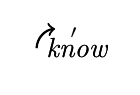
\begin{tikzpicture}[baseline]
    \qtreecentertrue \Tree [.IP \textit{I} [.I$'$ [.I \node(knowI){\textit{know}}; ] [.VP \textit{not} [.VP [.V \node(knowV){\textit{\sout{know}}}; ]]]]]
    \draw[thick] (knowV.west) edge [bend left=40,->] (knowI);
\end{tikzpicture}

\noindent\ex \label{ex:Knowyounot}
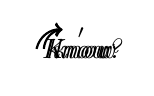
\begin{tikzpicture}[baseline]
    \Tree [.CP [.C \node(knowC){\textit{Know}}; ]
    [.IP \textit{you} [.I$'$ [.I \node(knowI){\textit{\sout{know}}}; ]
    [.VP (\textit{not}) [.VP [.V \node(knowV){\textit{\sout{know}?}}; ]
    ]]]]]
    \draw[thick] (knowV.west) edge [bend left=40,->] (knowI);
    \draw[thick] (knowI.west) edge [bend left=40,->] (knowC);
\end{tikzpicture}
\end{exe}
\end{multicols}

\noindent The loss of this V-to-I movement\is{V-to-I movement} is a long process, stretching from 1400 to 1800, and involving substantial variation both within and between individuals (see e.g. \citet{HaeberliIhsane2016} for details). At the same time as this fundamental change in the positioning of lexical verbs\is{syntactic trees} occurred, new auxiliaries were emerging. One of these is the emergence of what's called \textit{DO}-support.\footnote{Also known in the literature as \textsc{periphrastic} or \textsc{dummy} \textit{DO}.} The \textit{DO} of \textit{DO}-support, like the other auxiliaries, is an I element, and bears its name because it's semantically empty: it simply has to be inserted in order to form a negative\is{negation} statement or a question, as in the Present Day English trees (\ref{ex:Idonotknow}) and (\ref{ex:Doyounotknow}). Because this \textit{DO} is an I element, it exhibits the four NICE\is{NICE properties} properties discussed above.\is{syntactic trees}

\begin{multicols}{2}
\begin{exe}
\ex \label{ex:Idonotknow}
\begin{tikzpicture}[baseline]
    \Tree [.IP \textit{I} [.I$'$ [.I \textit{do} ] [.VP \textit{not} [.VP [.V \textit{know} ]]]]]
\end{tikzpicture}

\ex \label{ex:Doyounotknow}
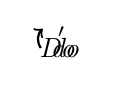
\begin{tikzpicture}[baseline]
    \Tree [.CP [.C \node(doC){\textit{Do}}; ] [.IP \textit{you} [.I$'$ [.I \node(doI){\textit{\sout{do}}}; ] [.VP (\textit{not}) [.VP [.V \textit{know?} ]]]]]]
    \draw[thick] (doI.west) edge [bend left=40,->] (doC);
\end{tikzpicture}
\end{exe}
\end{multicols}
\setlength{\columnsep}{10pt}

\noindent Among the Germanic languages, \textit{DO}-support is completely unique. In Old and Middle English, \textit{DO} was simply a lexical verb with the semantic content of `make' or `achieve' (as in e.g. \textit{I am doing my homework}). But what's striking when you compare the trees\is{syntactic trees} in (\ref{ex:Iknownot}) (Early Modern English) and (\ref{ex:Idonotknow}) (Present Day English) for negation,\is{negation} or in (\ref{ex:Knowyounot}) (Early Modern English) and (\ref{ex:Doyounotknow}) (Present Day English) for questions, is that \textit{DO} seems to play the same role as V-to-I movement: it fills the I ``slot''.\is{syntactic trees} If that's true, the rise of \textit{DO}-support should take place at the same time as the fall in V-to-I movement\is{V-to-I movement} -- and this seems to be correct \citep{Roberts1985,Roberts1993,Kroch1989}.\footnote{Why \textit{DO}, of all verbs, becomes an auxiliary with no semantic content is another question. One prominent suggestion is that influence from the Celtic languages of Britain (see \sectref{OE-Celtic}) may have played a role. Present Day \ili{Welsh} offers us sentences such as \textit{Dwi'n hedfan hefo alarchod} `I fly/I'm flying with swans', where the auxiliary verb \textit{BE} is the \textit{dwi} component in this case (`am', literally). The Welsh \textit{dwi} is phonologically quite close to the Present Day English \textit{DO}. See \citet{vanderAuweraGenee2002} for references and an evaluation.}

\begin{figure}
        \includegraphics[width=.75\textwidth]{chapters/img/ecay-do.png}
    \caption{The rise of \emph{DO}-support in a variety of linguistic contexts. The dip after 1575 is clearly visible. From \citet[54]{Ecay2015}, used with author's permission; data are taken from the Penn Parsed Corpora\is{corpora} of Historical English, replicating \citet{Ellegard1953}.}
    \label{fig:do}
\end{figure}

Sociolinguistic\is{sociolinguistics} and stylistic factors also play a role in the change. In negative\is{negation} declarative clauses like (\ref{ex:Iknownot}) and (\ref{ex:Idonotknow}), the use of \textit{DO}-support increases up until 1575, then levels out for a while (see Figure \ref{fig:do}). \citet{Warner2005} shows that, before 1575, texts that contain a more complex vocabulary also contain more \textit{DO}-support, but after 1600 the picture is reversed: texts with a more complex lexicon use less \textit{DO}-support. The rate of \textit{DO}-support increases steadily in texts with a less complex lexicon, but rises and then falls after 1575 in texts with a more complex lexicon. After 1600, older people also use \textit{DO} less. How to explain this? \citet{Warner2005} suggests that after 1600 a strong stylistic dispreference for \textit{DO}-support in higher register texts emerged. It's plausible to think that this is linked to the rise of a standard language ideology\is{standardization}\is{standard language ideology} (\sectref{EModE-standardization}) and of an increasingly judgemental behaviour around written norms during the same period: perhaps what was perceived as more formal/standard at the later stage reflected a ``pre-\textit{DO}'' stage.


\begin{syntaxbox}{The modals}
The core modals\is{modals} -- \textit{can}, \textit{could}, \textit{may}, \textit{might}, \textit{must}, \textit{shall}, \textit{should}, \textit{will}, and \textit{would} -- have properties in Present Day English that are odd even by auxiliary standards: for instance, they can't have non-finite forms (e.g. *\textit{I want to can}). See \sectref{ME-modals} of this book for discussion of the morphosyntactic properties of the modals, and also \sectref{LME-semimodals} on the more recently emerging ``semi-modals''.
\end{syntaxbox}


\noindent For more detail on the changes discussed in this subsection, and fuller versions of the arguments developed here, see \citet[Chapter 4, especially §4.6]{Los2015}.\is{auxiliaries|)}\is{\emph{DO}-support|)}

\subsection{Preposition stranding}\label{EModE-stranding}\is{preposition stranding|(}
\largerpage
Is a preposition something you'd end a sentence with? If not, what are you afraid of? Preposition stranding -- i.e. the placement of a preposition apart from, usually after, the noun phrase it belongs to -- is one of the grammatical features of English that prescriptivists\is{prescriptivism} most love to complain\is{complaint tradition} about \citep[107--115]{Crystal2006fight}. Nevertheless, it has been part of the English language since before the earliest texts were written.\footnote{Though not in exactly the same contexts in which it appears in Present Day English. See \citet[64--67]{Fischeretal2000} for a discussion of preposition stranding in Old English, and a syntactic analysis.} All three of the opening sentences of this paragraph contain preposition stranding. Here are some more examples from Early Modern English:

\begin{exe}
\ex Sulphur like unto the common one, and more combustible than perhaps you will at first take notice \textbf{of}\\
(Robert Boyle,\ia{Boyle, Robert} \textit{The Sceptical Chymist}, 1661)
\ex Oroonoko was first seized \textbf{on}, and sold to our overseer\\
(Aphra Behn,\ia{Behn, Aphra} \textit{Oroonoko}, 1688)
\ex The mawes, and dens of beasts could not receiue\\
The bodies, that those soules were frighted \textbf{from}\\
(Ben Jonson,\ia{Jonson, Ben} \textit{Catiline his Conspiracy}, 1611)\label{ex:stranding-jonson}
\ex What were you talking \textbf{of} when I came?\\
(Shakespeare,\ia{Shakespeare, William} \textit{Troilus and Cressida}, 1609)\label{ex:stranding-shakespeare}
\end{exe}

\noindent The more standard option for preposition placement is called \textsc{pied-piping}, and has the preposition next to its complement, e.g. \textit{Of what were you talking?}

Where did the proscription against stranded prepositions come from, then, and how did it enter into the standard language?\is{standardization} The first person to explicitly condemn stranding seems to have been John Dryden,\ia{Dryden, John} an English literary critic and poet.\is{poetry} In an essay of 1672 criticizing the ``errors'' of earlier writers, Dryden seizes upon example (\ref{ex:stranding-jonson}),\footnote{Ironically, Dryden actually makes an error in his citation of Jonson,\ia{Jonson, Ben} writing \textit{waves} rather than the original \textit{mawes}.} describing it as ``[t]he preposition in the end of the sentence; a common fault with him [Jonson], and which I have but lately observed in my own writings.'' When revising his own work after 1668, Dryden attempted to ``correct'' stranded prepositions (\citealp{Bately1964}; \citealp[157--158, 188--194]{YanezBouza2015}). Dryden also rewrote Shakespeare's\ia{Shakespeare, William} \textit{Troilus and Cressida}, a play which he described as a ``heap of Rubbish'', in 1679, and corrected \textit{talking of} in example (\ref{ex:stranding-shakespeare}) to \textit{a talking}.

Dryden clearly saw himself as someone trying to improve the English language. However, why Dryden disliked stranded prepositions so much, and considered them a ``fault'', is not entirely clear. \citet[275]{Bately1964} suggests that he is trying to ``force the mother tongue into a \ili{Latin} mould'': Latin does not allow separation of a preposition from the noun phrase that follows it.\footnote{Note that this is not a \textit{prescriptive} rule of Latin. Rather, \ili{Latin} native speakers (and writers) simply didn't strand prepositions, just as modern \ili{French} or \ili{German} or \ili{Czech} native speakers don't today. In these languages, we're talking about a part of the mental grammar that is largely below the level of consciousness, not a taught prescriptive rule. See \citet[75--83]{Freidin2019} for discussion of the difference.} Many writings on English grammar from the same period were heavily influenced by the regularities of Latin. But the fallacy in this way of thinking is patently obvious: English simply isn't \ili{Latin}.

The proscription against preposition stranding may originate with Dryden,\ia{Dryden, John} but makes its way into the standard as part of the process of codification (see \sectref{EModE-standardization})\is{standardization} during the eighteenth century. Robert Lowth,\ia{Lowth, Robert} who is known to have read Dryden, discusses stranding in his extremely influential 1762 \textit{Short Introduction to English Grammar}, and says the following \citep[127--128]{Lowth1762}:

\begin{quote}
    [Stranding] is an Idiom, which our language is strongly inclined to; it prevails in common conversation, and suits very well with the familiar style in writing; but the placing of a Preposition before the Relative\is{relative clauses} is more graceful, as well as more perspicuous; and agrees much better with the solemn and elevated Style.
\end{quote}

\noindent ``Bishop Lowth''\ia{Lowth, Robert} has been demonized as the arch-prescriptivist,\is{prescriptivism} but more recent research has shown that this is not really fair (\citealp[111]{Beal2004}; \citealp{Tieken2010}). In this quote we see Lowth making a distinction between speech and writing, and between ``familiar'' and ``solemn'' styles \citep[214--218]{YanezBouza2015}. 

\begin{wrapfigure}{r}{0.35\textwidth}
        \includegraphics[scale=0.17]{chapters/img/Robert_Lowth_portrait.jpg}
    \caption{Robert Lowth}
    \label{fig:Lowth}
\end{wrapfigure}

\hspace*{-5pt}Lowth also uses stranding himself here (``strongly inclined \textbf{to}''). Still, Lowth gives no reason for considering stranding to be less graceful or perspicuous. And all of the nuance in Lowth's careful statement is stripped out by later grammarians, who adopt much of Lowth's work almost verbatim (norms around authorship, attribution, and plagiarism were not the same in the eighteenth century as they are today). \citet[218]{YanezBouza2015} is able to trace Lowth's influence in twenty different texts by fifteen different authors of the period. Lindley Murray's\ia{Murray, Lindley} (1795) \textit{English Grammar} is one notable example, reproducing Lowth's text almost exactly but changing the text to get rid of the stranding (``an idiom \textbf{to which} our language is strongly inclined''). Traces of Lowth's\ia{Lowth, Robert} passage can also be found in the works of the female grammarians of the period, such as Ellin Devis.\ia{Devis, Ellin}

Dryden's\ia{Dryden, John} and Lowth's\ia{Lowth, Robert} remarks and the codification of stranding as outside the standard\is{standardization} had a real effect on usage. \citet[chapter 4]{YanezBouza2015} and \citet{Sairio2009} show that the frequency\is{frequency} of preposition stranding in written texts sinks dramatically during the second half of the eighteenth century, even in the usage of individuals over their lifespan. Still, preposition stranding is alive and well in Present Day English, even if still frowned upon by some prescriptive authorities, suggesting that even the strongest prescriptive condemnation is unlikely to extirpate a syntactic feature entirely.\is{word order|)}\is{preposition stranding|)}

\section{Lexicon}\label{EModE-lexicon}
Three phenomena are particularly noteworthy when it comes to the lexicon of Early Modern English. Two are related to borrowings:\is{borrowings} as we saw in \sectref{EModE-history}, Early Modern English is marked by English becoming standardized\is{standardization} and by colonization.\is{colonialism} The former, as we shall see here, is closely tied to lexical borrowings\is{borrowings} from \ili{Latin}, \ili{French}, and \ili{Greek}, and caused quite a stir-up at the time (the so-called inkhorn controversy).\is{inkhorn controversy} The latter meant that English speakers came into contact with speakers of many other languages, on an unprecedented scale at the time. Finally, when contrasted with the older periods, Early Modern English saw a rise in a \glossterm{gl-derivation}{derivational} process called conversion.\is{conversion} Let's have a look at these one by one in what follows.


\subsection{Conversion}\label{EModE-conversion}\is{conversion|(}
\largerpage[2]
We have seen a process known as conversion already in Chapters \ref{introduction} and \ref{englishtoday}. It is also known as zero shift, functional shift, or zero derivation (or a \glossterm{gl-derivation}{derivation} by a zero \glossterm{gl-morpheme}{morpheme}, to add one more term to the menagerie). Conversion involves a process whereby a word of a specific word class is used as a word of another word class without its structure being changed in any way. For instance, the word
\textit{bottle} would come to our mind most likely as a noun by default, as in \textit{There's a \textbf{bottle} on the table}. However, if we put this word in a different syntactic context, it becomes a verb, as in {\textit{Let's \textbf{bottle} some wine!}} and \textit{She had been \textbf{bottl}ing wine for as long as she could remember, introduced to the art by her father.}\footnote{OED, \glossterm{gl-sv}{s.v.} bottle, v.1.}

We can find some remarkable cases of conversion already in Early Modern English, e.g. in Shakespeare's\ia{Shakespeare, William} \textit{\textbf{Grace} me no grace, nor \textbf{uncle} me no uncle} from \textit{Richard II}, where the nouns \textit{grace} and \textit{uncle} are unconventionally used also as verbs. In Present Day English, we can occasionally find even entire clauses used as verbs or modifiers, as in \textit{``Don't ``I told you so'' me,'' Martin snapped.} \citep{Clark2016}.

This has nevertheless not always been the case throughout the earlier history of the English language. This word-formation strategy became ``the third most common way of expanding the vocabulary'' only in the period of 1500--1700 \citep[283]{MillHay2018}, following affixing\is{affixes} and \glossterm{gl-compounding}{compounding}.\is{word formation}


\begin{miscbox}{I'd be bumblebeed}
\is{bumblebees}
Some internet searching gives us cases of conversions\is{word formation} such as the following:\footnote{\url{https://www.navitron.org.uk/forum/index.php?topic=7443.15}.}
\begin{itemize}
    \item \textit{however we were now short of a header tank for the heating/stove and as its 40 miles to town I was \textbf{bumblebeed} if I was going to buy one} [...]
\end{itemize}
The word \textit{bumblebee}, historically and by default used as a noun, can apparently also be used as a verb, albeit extremely marginally so. Well, I'd sure be bumblebeed...\is{conversion|)}
\end{miscbox}


\subsection{Colonial borrowings}\is{colonialism|(}\is{borrowings|(}

\sloppy
\begin{wrapfigure}{l}{0.45\textwidth}
        \includegraphics[scale=0.5]{chapters/img/668px-Wombat_1.jpg}
    \caption{Wombat: a marsupial native to Australia (photo by Stygiangloom, licensed under CC-BY 2.0)}
    \label{fig:Wombat}
\end{wrapfigure}

Encounters with new cultures and new fauna and flora typically require new labels for new concepts. These concepts are typically nouns (e.g. a wombat, a rather cute marsupial native to Australia; see Figure \ref{fig:Wombat}), which makes sense considering new labels are typically needed for fairly specific objects, unknown to the explorers.

If we use the advanced search option in the Oxford English Dictionary\is{dictionaries} and limit our search to loans from Australian Aboriginal languages between the years of 1500--1700, we find no results. Considering what we said about the history of Australian English (in the box in \sectref{English-NA}), this makes sense: Anglophone presence in Australia dates back to 1788. It therefore also makes sense that extending the period to 1800 produces 11 loanwords, such as \textit{dingo} and \textit{wombat} (from \ili{Dharug}) and \textit{kangaroo} (from \ili{Guugu Yimidhirr}). Ten of these are nouns and ten refer to the fauna and flora of Australia, and Australian culture. This trend is confirmed by searches restricted to other groups of non-European languages: loanwords are often nouns necessary to label newly encountered objects and entities.

Searching within 1500--1700, we get 46 loans from Austronesian languages of the Asia-Pacific region and Oceania, all of which are nouns (three of these are nouns as well as another word class). One Austronesian loan is \textit{babirusa}, `a long-legged wild pig', from \ili{Malay}. Considering the longer colonial history in North America (in contrast to Australia), it is not surprising that Native American languages give us 106 results. Of these, all can function as nouns, and some as other word classes as well. Some of these loans include \emph{maize} and \emph{potato} (both from \ili{Taíno} via Spanish), \emph{tomato} (from Nahuatl via Spanish), \textit{jaguar}, \textit{moccasin}, \textit{moose}, \textit{raccoon}, \textit{squash}, and \textit{terrapin}. Limiting the search to contact with languages of the Indian subcontinent, 239 results are provided. This high number also makes sense: the Indian subcontinent was heavily exploited by the colonizers. Again, all but three of these loans can function as nouns. Some of these include \textit{Buddha} (from \ili{Pali}), \textit{dungaree}, \textit{ghee}, \textit{guru}, \textit{pukka}, \textit{pundit}, and \textit{yogi} (from \ili{Hindi/Urdu}), and \textit{mongoose} (from \ili{Telugu} via \ili{Portuguese}). Central and Eastern Asian languages result in 131 entries, including for instance \textit{baklava}, \textit{harem}, and \textit{yoghurt} (from \ili{Turkish}), \textit{cha} (related to Present Day English \textit{chai} and \textit{tea}; from \ili{Chinese}), \textit{Islam} (from \ili{Arabic}), \textit{jackal} (from \ili{Persian} and \ili{Turkish}), \textit{ketchup}, \textit{litchi} and \textit{kumquat} (from \ili{Chinese}), \textit{lama} (from \ili{Tibetan}), \textit{soy} (from \ili{Japanese}), and \textit{tulip} (multiple languages). Middle Eastern and Afro-Asiatic languages lead to 357 entries and African languages give us 15 loans (such as \textit{okra}, a type of edible plant, from a Niger-Congo language, probably \ili{Igbo}).

These trends are by no means limited to Early Modern English. If we did similar searches for the languages relevant for Late Modern English or Present Day English, we would also find plenty of borrowings necessary for unknown objects, perfectly known in the newly explored locales. Typically, as we shall see in the chapters to follow, the type of linguistic materials borrowed from a language depends on the nature of the cultural contact and very much on the situational power relationships. Studying where which words come from can thus provide interesting evidence related to the relationships of different cultures through times.\is{colonialism|)}


\subsection{Latin and Greek borrowings: the inkhorn controversy}\il{Latin|(}\il{Greek|(}\is{inkhorn controversy|(}

By the start of the Early Modern period in 1500, the Renaissance\is{Renaissance} was in full flow in Europe. A philosophical movement originating in what is now Italy, the intellectual roots of the Renaissance were in Classical Latin and Greek thought, particularly the Greek philosophers, who had been ``rediscovered'' in Europe shortly before. Its effect upon the intelligentsia of early modern Europe was profound: from 1450 onwards, universities began to spring up in great numbers all around Europe.

Comparison with Latin and Greek no doubt played an important role in the emerging standardization\is{standardization} of the modern languages of Europe. In the lexicon of English, this is particularly evident in the borrowing of many new words from Latin and Greek during the Early Modern period. According to the data from the third edition of the Oxford English Dictionary\is{dictionaries} in \citet[23--28]{Durkin2014}, Latin is by far the most prolific donor language in the history of English to date, responsible for over thirteen thousand borrowings into English.\footnote{The total number of headwords in the OED3 is 92,500.} English has always borrowed words from Latin, but the peak of these borrowings is just after 1600.\footnote{If you have access, you can check this for yourself at \url{http://www.oed.com/timelines}.} Greek, meanwhile, is in third place after \ili{French} (on which see \sectref{ME-French-borrowing} in the next chapter), responsible for well over two thousand borrowings, almost all dating to after 1500. Together, Latin and Greek account for over half of all lexical borrowings in the history of English. Admittedly, the vast majority of these Latin and Greek borrowings are highly learned and/or technical terms which only appear very rarely and in specific registers. Nevertheless, the impact of these classical languages on the lexicon of English during the Early Modern period was clearly immense. The second half of the seventeenth century saw more borrowings enter English than any other period in history \citep[299--301]{Durkin2014}. Perhaps even more strikingly, these new Latin and Greek words were ready input to further word-formation processes, which continued robustly in English during the nineteenth and twentieth centuries, especially in the scientific\is{scientific language} domain \citep[340--347]{Durkin2014}.

\begin{table}
    \caption{Some borrowings from Latin in Early Modern English \citep[chapter 14]{Durkin2014}}\label{tab:EModE-borrowings}
  \begin{tabularx}{.8\textwidth}{XXl}
    \lsptoprule
    celebrate & communicate & contemplate \\
    describe & fact & frivolous \\
    national & pulsate & reconciliatory\\
    resonate & subsidiary & supervise\\
    \lspbottomrule
  \end{tabularx}
\end{table}

As we've seen in the section on standardization\is{standardization} (\sectref{EModE-standardization}), one of the processes involved is \textsc{elaboration}: the new standard language is used in new domains, or used increasingly in domains where other languages were dominant, and this brings with it a need for new words. These words can be formed using the language's own word-formation strategies, such as conversion\is{conversion} (\sectref{EModE-conversion} above), or they can simply be borrowed. Since the discourse in many of these new domains was previously dominated in usage by Latin in particular, borrowing words from Latin was the most obvious fix.

This influx of borrowings from classical languages did not sit well with everyone. The incipiently standardizing\is{standardization} English language was becoming a source of pride: headmaster Richard Mulcaster\ia{Mulcaster, Richard} commented in 1582 that ``I take this present period of our English tung to be the verie height thereof''. Mulcaster also commented on the number of words being borrowed into the language, ``either of pure necessitie in new matters, or of mere brauerie, to garnish it self withall''. Here \textit{brauerie} means `showiness' or `ostentatiousness', implying that some of these borrowings were for reasons of fashion, not because they were needed. The prestige\is{prestige} of classical languages meant that using Latin and Greek words in English could be taken as a mark of education, or of (perceived) social superiority. In turn, people could be mocked for this. The teacher Holofernes in Shakespeare's\ia{Shakespeare, William} \textit{Love's Labours Lost} peppers his language liberally with Latin and Latinisms (e.g. when reading a letter, he says ``I will \textbf{overglance} the \textbf{superscript}''), and is intended as a figure of ridicule. Thomas Wilson's\ia{Wilson, Thomas} influential \textit{Arte of Rhetorique} (1553) puts it like this:

\begin{quote}
    Among all other lessons this should first be learned, that wee neuer affect any straunge ynkhorne termes, but to speak as is commonly received ... Some seeke so far for outlandish English, that they forget altogether their mothers language.
\end{quote}

\noindent Wilson\ia{Wilson, Thomas} writes of ``inkhorn terms'', which became a catchphrase for Latin and Latinate words that were perceived to be unnecessary or affected. This influenced the first generation of dictionaries\is{dictionaries} in the seventeenth century, such as Thomas Blount's\ia{Blount, Thomas} (1656) \textit{Glossographia}: these works were lists of explanations of words thought to be difficult, not dictionaries\is{dictionaries} in the sense we're more familiar with today. Although it's easy to laugh at the supposed pretentiousness of the Early Modern writers criticized, the darker side of the inkhorn controversy is linguistic \glossterm{gl-purism}{purism}\is{purism} \citep{Thomas1991,LangerNesse2012}, the desire to preserve languages from foreign elements, and the view that inherited words are better than borrowed ones. Linguistic purism\is{purism} goes hand in hand with standard language ideology\is{standardization}\is{standard language ideology} and with ethnonationalism,\is{nation-states} and so it is not surprising to see it on show in the Early Modern period.

The critics of inkhorn terms were not, on the whole, successful in suppressing Latin words. All of the words in Table \ref{tab:EModE-borrowings} are still found in English today, with no particular negative connotations. Still, in some quarters the sentiment behind the inkhorn critics persists. As recently as 1946, George Orwell's\ia{Orwell, George} essay \textit{Politics and the English Language} complains\is{complaint tradition} that ``unnecessary words like \textit{expedite}, \textit{ameliorate}, \textit{predict}, \textit{extraneous}, \textit{deracinated}, \textit{clandestine}, \textit{subaqueous}, and hundreds of others constantly gain ground from their Anglo-Saxon opposite numbers''. Needless to say, Orwell\ia{Orwell, George} provides no evidence for this claim, nor any argument for the superiority of their inherited Germanic ``opposite numbers''.\footnote{For more on the inkhorn controversy, see \url{https://shakespeareandbeyond.folger.edu/2019/04/05/inkhorn-controversy-latin-greek-english-words/} and \citet[Chapter 2]{Barber1997} -- also make sure to have a go at Exercise \ref{EModE-inkhorn-exercise}!}\il{Latin|)}\il{Greek|)}\is{borrowings|)}\is{inkhorn controversy|)}

\section{Final note}

It's the Early Modern period more than any other that explains how and why the English language got to where it is today -- both in terms of its geographical distribution and its social status. We've seen that the process of standardization\is{standardization} -- closely linked to the rise of nationalism\is{nation-states} -- really took off during this period, as did the spread of English worldwide via colonialism and imperialism.\is{colonialism}\is{British Empire} Some of the linguistic changes we see during this period are also connected to this emerging sense of British self-importance: the rise of borrowings\is{borrowings} from the prestige\is{prestige} languages Greek and Latin (and the pushback against these borrowings)\is{borrowings} is a case in point. But, just like in every other period, we also see structural changes that bear no obvious relation to social or cultural developments, such as the rise of \emph{DO}-support\is{\emph{DO}-support} and the Great Vowel Shift.\is{vowels}\is{Great Vowel Shift} These are good indications that standardization\is{standardization} -- for all its centrality to the way we think about language today -- can never prevent a language from developing in new and unexpected ways.


\addsec{Suggested exercises}

\begin{exercises}{Reflexes of the Great Vowel Shift}\label{EModE-GVS-exercise}\label{ex-GVS}\is{Great Vowel Shift|(}
You\is{vowels|(} will be using a dataset created as part of the project called ``Seeing Speech'' \citep{LawsonEtAl2015}.\footnote{The dataset is available here: \url{https://www.dynamicdialects.ac.uk/accent-chart/}.}\\

\noindent A.\\
Listen to the production of FACE, GOAT, MOUTH of the speakers from the following places:\is{regional variation}
 
\begin{enumerate}
    \item Greater Manchester 
    \item Kent 
    \item London 
    \item Newcastle 
    \item North Yorkshire 
    \item Co. Tipperary 
    \item Orkney 
    \item Perthshire
\end{enumerate}

\noindent Note whether the vowel is a monophthong, a diphthong,\is{diphthongization} or somewhere in between. Is it always easy to decide?\\

\noindent B.\\
Which of these speakers show more conservative vowel features? In other words, which speakers' accents reflect older stages of the language?\\

\noindent\emph{Tip for the teachers:} This can be assigned as a written exercise practising summarizing skills. Give the students a maximum word count and a deadline for the written exercise.\\

\noindent\emph{Tip for the students:} If you're asked to submit your answers as a written assignment, your answer should be structured as follows: 1. What's the question/problem? (setting up the context); 2. Show us how you answer this question/tackle the problem. (argumentation); 3. What's your answer/conclusion? (sum up clearly)\is{vowels|)}\is{Great Vowel Shift|)}

\end{exercises}

\begin{exercises}{For I thou thee, thou traitor!}\label{ex-thou}\is{T-V system (pronouns)|(}
Look at the 2nd person pronouns in the two passages below. The pronouns are highlighted for you. The first passage comes from the \textit{Trial of Sir Walter Raleigh, Knight, for High Treason, by a Special Commission of Oyer and Terminer, at Winchester, 17th November, 1603. 2 James I} \citep[408--410]{Jardine1832}. The second bunch of excerpts is taken from Shakespeare's\ia{Shakespeare, William} \textit{Hamlet}. We give you a snippet of a conversation between Hamlet and the Queen, his mother, and also a conversation between Hamlet and the Ghost, who turns out to be his dead (murdered) father. Your tasks are presented following the excerpts.\footnote{These passages are taken from the following Project Gutenberg webpage, accessed in February 2020: \url{https://www.gutenberg.org/files/1524/1524-h/1524-h.htm}.}\\

\noindent A.
\begin{quote}
    \textbf{Sir Walter Raleigh.} All this while \textbf{you} tell me news, Mr. Attorney.
    
    \textbf{Attorney General.} Sir Walter, I cannot blame \textbf{you}, though \textbf{you} be moved.
    
    \textbf{Sir Walter Raleigh.} Nay, \textbf{you} fall out with \textbf{yourself}; I have said nothing to \textbf{you}; I am in no case to be angry.

    [...]

    \textbf{Attorney General.} After Raleigh understood that he was accused by my Lord Cobham, it was contrived that the Lord Cobham should retract his accusation, and that he might make his retraction known and believed, the course was this: [...]. Came this contrivance, think \textbf{you}, out of Cobham's quiver? No, but out of Raleigh's devilish and Machiavelian policy. \textbf{You} shall hear that it was after Cobham had had intelligence with this viper in the Tower, that he devised this false artifice. But Sir Thomas Fane would be no party in such a business, and sent the letter to the Council.
    
    \textbf{Sir Walter Raleigh.} What is that to me? I do not hear yet that \textbf{you} have spoken one word against me; here is no treason of mine done; if my Lord Cobham be a traitor, what is that to me?
    
    \textbf{Attorney General.} All that he did was by \textbf{thy} instigation, \textbf{thou} viper, for I \textbf{thou} \textbf{thee}, \textbf{thou} traitor! I will prove \textbf{thee} the rankest traitor in all England.
    
    \textbf{Sir Walter Raleigh.} No, no, Mr. Attorney, I am no traitor. Whether I live or die, I shall stand as true a subject as any the King hath; \textbf{you} may call me traitor at your pleasure; yet it becomes not a man of quality and virtue to do so; but I take comfort in it, it is all that \textbf{you} can do, for I do not yet hear that \textbf{you} charge me with any treason.
    
    \textbf{Lord Chief Justice.} Sir Walter Raleigh, Mr. Attorney speaks out of the zeal of his duty for the service of the King; and \textbf{you} for your life; be patient on both sides.
\end{quote}

\noindent B.
\begin{quote}
    \textbf{QUEEN.} Let not \textbf{thy} mother lose her prayers, Hamlet. I pray \textbf{thee} stay with us; go not to Wittenberg.
    
    \textbf{HAMLET.} I shall in all my best obey \textbf{you}, madam.\\

    [...]\\

    \textbf{HAMLET.} Angels and ministers of grace defend us! Be \textbf{thou} a spirit of health or goblin damn'd, Bring with \textbf{thee} airs from heaven or blasts from hell, be \textbf{thy} intents wicked or charitable, \textbf{thou} com'st in such a questionable shape that I will speak to \textbf{thee}. [...] What may this mean, that \textbf{thou}, dead corse, again in complete steel, [...] say, why is this? Wherefore? What should we do?
    
    \textbf{HORATIO.} It beckons \textbf{you} to go away with it, as if it some impartment did desire to \textbf{you} alone.\\

    [...]\\

    \textbf{HAMLET.} Whither wilt \textbf{thou} lead me? Speak, I'll go no further.
    
    \textbf{GHOST.} Mark me.
    
    \textbf{HAMLET.} I will.
    
    \textbf{GHOST.} My hour is almost come, when I to sulph'rous and tormenting flames must render up myself.
    
    \textbf{HAMLET.} Alas, poor ghost!
    
    \textbf{GHOST.} Pity me not, but lend \textbf{thy} serious hearing to what I shall unfold.

    \textbf{HAMLET.} Speak, I am bound to hear.

    \textbf{GHOST.} So art \textbf{thou} to revenge, when \textbf{thou} shalt hear. [...] I am \textbf{thy} father's spirit, doom'd for a certain term to walk the night, [t]ill the foul crimes done in my days of nature are burnt and purg'd away. [...] List, list, O, list! If \textbf{thou} didst ever \textbf{thy} dear father love—
    
    \textbf{HAMLET.} O God!

    \textbf{GHOST.} Revenge his foul and most unnatural murder.
    
    \textbf{HAMLET.} Murder! [The Ghost/Father tells him how he was murdered by Hamlet's uncle, the Ghost's/former King's brother.] O my prophetic soul! Mine uncle!
    
    \textbf{GHOST.} Ay, that incestuous, that adulterate beast, with witchcraft of his wit, with traitorous gifts,— o wicked wit, and gifts, that have the power so to seduce!—won to his shameful lust the will of my most seeming-virtuous queen. [...] Adieu, adieu, adieu. Hamlet, remember me.
    
    \textbf{HAMLET.} O all \textbf{you} host of heaven! O earth! What else? And shall I couple hell? O, fie! Hold, my heart; And \textbf{you}, my sinews, grow not instant old. But bear me stiffly up. Remember \textbf{thee}? Ay, \textbf{thou} poor ghost, while memory holds a seat in this distracted globe. Remember \textbf{thee}?
\end{quote}

\noindent And here are your tasks:

\begin{enumerate}
\item Identify instances where the same speaker switches from \textit{you} (or \textit{yourself}) to \textit{thou} (or \textit{thyself} or \textit{thee}), and the other way round. Why do you think these switches take place?
\item Looking beyond pronouns, how do the speakers address each other? Give specific noun phrases (e.g. \textit{lovely bumblebee})\is{bumblebees} or determiner phrases (e.g. \textit{my precious jewel}). Are these forms of address negative, positive, or neutral? Can this help to shed any light on the pronominal switches you've identified?
\item The Chief Lord of Justice makes a mention of the emotional state of the Attorney General. How does this relate to the pronominal switches, if at all?
\item This time you were given fairly long passages to look at. Why weren't you given just those sentences that contain 2nd person pronouns?\is{T-V system (pronouns)|)}
\end{enumerate}

\end{exercises}

\begin{exercises}{Shakespearean syntax}\label{exercise-shakespeare-syntax}\is{word order|(}
Examine the Shakespearean\ia{Shakespeare, William} quotations below and describe how they differ from Present Day English morphologically and syntactically. Pay particular attention to what the finite verb is doing.

\begin{enumerate}
    \item \emph{What says he of our marriage? What of that?} (Romeo and Juliet 2.5)
    \item \emph{Put up your swords; you know not what you do.} (Romeo and Juliet 1.1)
    \item \emph{A crutch, a crutch! why call you for a sword?} (Romeo and Juliet 1.1)
    \item \emph{O, where is Romeo? saw you him to-day?} (Romeo and Juliet 1.1)
    \item \emph{Fear me not.} (Romeo and Juliet 1.1)
\end{enumerate}

\end{exercises}

\begin{exercises}{Preposition stranding in your own daily life?}\is{preposition stranding|(}

\begin{enumerate}
    \item Find 3 examples of preposition stranding
    \begin{itemize}
        \item on the social media\is{media} you engage with
        \item in spoken interactions you have with others
    \end{itemize}
    \item Was it difficult to find these 3 examples for each context?
    \item Now rewrite these examples so that they don't contain any preposition stranding.
    \item Finally, try this exercise in reverse! Find three examples of pied-piping -- perhaps in academic articles or textbooks. Now rewrite them so that they contain preposition stranding!
\end{enumerate}

\noindent\emph{Acknowledgement:} this exercise was suggested to us by Nicole Tamer.\is{word order|)}\is{preposition stranding|)}

\end{exercises}

\begin{exercises}{Whence synonymity?}\label{exercise-synonymity}
The following 20 words represent 10 pairs of synonyms. You need to identify these 10 pairs:

\begin{quote}
    \textit{bless}, \textit{break}, \textit{chew},  \textit{cogitate}, \textit{consecrate}, \textit{depart}, \textit{disintegrate}, \textit{drink}, \textit{emancipate},  \textit{flood}, \textit{free}, \textit{go}, \textit{imbibe}, \textit{inundate}, \textit{job}, \textit{lie}, \textit{masticate}, \textit{position}, \textit{prevaricate}, \textit{think}
\end{quote}

\noindent One word in each pair is \ili{Latin}- or \ili{French}-derived and one is Germanic. Sort the individual words into two categories: one with all the Germanic words and one with all the Romance words. 

\begin{enumerate}
\item What differences (e.g. number of syllables, semantics, etc.) do you notice between the two sets?
\item Discuss the language styles in which the use of one or the other is more appropriate.
\end{enumerate}

\noindent \emph{Acknowledgement:} this exercise was taken and slightly adapted from Johanna Wood's\ia{Wood, Johanna L.} 2016 teaching materials.

\end{exercises}

\begin{exercises}{Irregular plurals in Present Day English}\label{exercise-irregular-plurals}\is{inflection}\is{irregularities}\is{plurals}
Sometimes borrowed\is{borrowings} words keep their foreign plurals. This often happens with \ili{Latin} and \ili{Greek} words used in specialized areas by educated people. Among such loan words are the following:

\begin{quote}
    \textit{analysis}, \textit{cherub}, \textit{index}, \textit{matrix}, \textit{medium}, \textit{nucleus}, \textit{species}, \textit{stigma}, and \textit{stratum}
\end{quote}

\noindent For each, give the foreign plural and the language from which it derives. (You will need a good dictionary,\is{dictionaries} such as the online OED.)

Sometimes two different plural forms may be used with different functions. Are you aware of any of these words above using both a regular and irregular\is{irregularities} plural\is{plurals} with different meanings?

\end{exercises}

\begin{exercises}{Inkhorn controversy}\label{EModE-inkhorn-exercise}\is{inkhorn controversy|(}
\emph{Note: for this exercise you will need access to the online Oxford English Dictionary\is{dictionaries} (OED) via your library or university.}\\

\noindent In 1557, Sir John Cheke\ia{Cheke, John} wrote the following:\is{purism}
 
\begin{quote}
    I am of this opinion that our own tung shold be written cleane and pure, unmixt and unmangeled with borowing of other tunges, wherin if we take not heed by tiim, ever borowing and never payeng, she shall be fain to keep her house as bankrupt. For then doth our tung naturallie and praisablie utter her meaning, when she bouroweth no counterfeitness of other tunges to attire her self withall, but useth plainlie her own, ... and if she want at ani tiim (as being unperfight she must) yet let her borow with suche bashfulness, that it mai appear, that if either the mould of our own tung could serve us to fascion a woord of our own, or if the old denisoned wordes could content and ease this neede, we wold not boldly venture of unknowen wordes. (in \citealp[31]{Wells1973})
\end{quote}
		
\noindent Look up the etymology of the following words in the OED: \textit{opinion}, \textit{clean}, \textit{pure}, \textit{unmixed}, \textit{unmangled}, \textit{borrow}, \textit{tongue}, \textit{never}, \textit{paying}, \textit{fine}, \textit{keep}, \textit{house}, \textit{bankrupt}.

Having looked up the etymology, what would you say to Sir John Cheke\ia{Cheke, John} as a trained linguist?\is{inkhorn controversy|)}\is{purism}

\end{exercises}

\begin{exercises}{Food for thought}
\begin{itemize}
    \item If the English spelling was reformed so that the grapheme-phoneme correspondence was a 1:1 correspondence, what immediate pros and cons would we have to deal with and why?\is{orthography}
    \item Which English accent should a spelling reform be based on and why?\is{orthography}
    \item Are chain shifts\is{chain shifts} such as the Northern Cities Shift\is{Northern Cities Shift} or the Short Front Vowel\is{vowels} Lowering\is{vowel lowering} to blame for the inconsistencies in Present Day English spelling?\is{orthography}
    \item Find a speaker of a language with T and V pronouns\is{pronouns} (widely-spoken languages with a T-V distinction include \ili{Bengali}, \ili{Chinese}, \ili{French}, \ili{Hindi/Urdu}, \ili{Russian}, \ili{Spanish}, and some varieties of \ili{Arabic}). Try to understand how their T-V distinction works. Is the distinction a useful one? Why (or why not)?\is{T-V system (pronouns)}\is{pronouns}
\end{itemize}

\end{exercises}

\begin{exercises}{Investigating \textit{y'all}, \textit{youse}, \textit{you guys}, and \textit{you lot}}\is{pronouns|(}
\chili{}

As mentioned in the chapter, new second person plural\is{plurals} forms have recently emerged, such as \textit{y'all}, \textit{youse}, \textit{you guys}, and \textit{you lot}. How would you design a project whose aim would be answering one of the following questions?
\begin{itemize}
    \item How old is the 2nd person pronoun construction?
    \item Is it used in a specific region?\is{regional variation}
    \item Is it used by a specific generation?
    \item Is it sex and/or gender sensitive?\is{gender studies}
    \item Is the pronoun stigmatized in any way, or is it viewed positively?
\end{itemize}

\noindent When thinking about your project design, consider the type of language you'd analyse (e.g. spoken, written, formal, informal), and whether you'd have to collect your own data (and how you would do that) or whether you could use already existing materials (corpora,\is{corpora} evidence online, etc.). Don't be afraid of the power of imagination!\is{pronouns|)}
\end{exercises}

\begin{texts}{A narrative of the captivity and removes of Mrs Mary Rowlandson}\label{EModE-Robinson-text}

Captivity narratives were a popular genre of literature in colonial North America.\is{colonialism} Here, Mary Rowlandson\ia{Rowlandson, Mary} (c. 1637--1711) describes her capture by Native Americans (she was later ransomed and released). Texts like these are useful as sources on Native Americans and their encounters with the colonists at the time, though they are far from neutral, and tell us as much if not more about the Puritan morality of the writers.\footnote{The text is taken from the \emph{Emerging Voices} \glossterm{gl-corpus}{corpus}\is{corpora} \citep{Walkden2019}, and is originally from the 1791 edition available at \url{https://archive.org/details/narrativeofcapti00inrowl/}, pp. 3--5.}

\begin{textglossed}
    \internallinenumbers*{}
    ON the 10th of \emph{February}, 1675, came the Indians with great numbers upon \emph{Lancaſter}: their firſt coming was about ſun-riſing; hearing the noiſe of ſome guns, we looked out: ſeveral houſes were burning and the ſmoke aſcending to heaven. There were five perſons taken in one houſe, the father and mother, and a ſucking child they knocked on the head, the other two they took and carried away alive. There were two others, who being out of their garriſon upon occaſion, were ſet upon; one was knocked on the head, the other eſcaped: Another there was who running along was ſhot and wounded, and fell down; he begged\marginnote{begged them to let him live} of them his life, promiſing them money (as they told me) but they would not hearken\marginnote{\emph{hearken}: listen; stripped} to him, but knocked him on the head, ſtript him naked, and ſplit open his bowels. Another ſeeing many of the \emph{Indians} about his barn, ventur'd and went out, but was quickly ſhot down. There were three others belonging to the ſame garriſon who were killed; the \emph{Indians} getting up upon the roof of the barn, had advantage to ſhoor\marginnote{\emph{ſhoor}: shower} down upon them over their fortification. Thus theſe \marginnote{murderous}murtherous wretches went on burning \& deſtroying all before them.
%     \end{linenumbers}
    
    ...
    
%     \begin{linenumbers}
    Then I took my children (and one of my ſiſters her's) to go forth and leave the houſe: but as ſoon as we came to the door, and appear'd, the \emph{Indians} ſhot ſo thick, that the bullets rattled againſt the houſe, as if one had taken a handful of ſtones and threw them, ſo that we were forced to give back. We had ſix ſtout dogs belonging to our garriſon, but none of them would ſtir\marginnote{\emph{ſtir}: move} though at another time, if an \emph{Indian} had come to the door, they were ready to fly upon him and tear him down. The Lord hereby would make us the more to acknowledge his hand, and to ſee that our help is always in him. But out we muſt go, the fire increaſing, and coming along behind us roaring, and the \emph{Indians} gaping before us with their guns, ſpears, and hatchets to devour us.
%     \end{linenumbers}

    ...
    
%     \begin{linenumbers}
    My eldeſt ſiſter being yet in the houſe and ſeeing thoſe \marginnote{\emph{woeful}: awful; \textit{halling}: hauling}woeful ſights, the infidels halling mothers one way and children another, and ſome wallowing in their blood: And her eldeſt ſon telling her that her ſon \emph{William} was dead, and myſelf was wounded, ſhe ſaid, and \emph{Lord let me die with them}: which was no ſooner ſaid. but ſhe was ſtruck with a bullet, and fell down dead over the threſhold. I hope ſhe is reaping the fruit of her good labours, being faithful to the ſervice of God in her place. In her younger years ſhe lay under much trouble upon ſpiritual accounts, till it pleaſed God to make that precious ſcripture take hold of her heart, \emph{3 Cor. 12. 9. And he ſaid unto me, My grace is ſufficient for thee.} More than twenty years after, I have heard her tell how ſweet and comfortable that place was to her. But to return; The \emph{Indians} laid hold of us, pulling me one way, and the children another, and ſaid, \emph{Come, go along with us}: I told them they would kill me; they anſwered, \emph{If I were willing to go along with them, they would not hurt me.}
%     \end{linenumbers}
\end{textglossed}


\end{texts}

\begin{texts}{Anne Bradstreet, \emph{A Dialogue between Old England and New}}\is{poetry|(}

Anne Bradstreet\ia{Bradstreet, Anne} (1612--1672) has the distinction of being the first published writer of the English colonies in North America. Born in England to a well-off family, she emigrated\is{migration} to America in 1630, where she remained for the rest of her life, becoming a poet widely read on both sides of the Atlantic.

This poem, written in 1642 and taken from her collection \emph{The tenth muse lately sprung up in America}, has as its subject matter the unease that was to lead to the English Civil War. An extract is presented here.\footnote{From \url{https://quod.lib.umich.edu/e/eebo2/A77237.0001.001/1:11?rgn=div1;view=fulltext}, pp186--187, accessed May 2020.}

\begin{textglossed}
    \internallinenumbers*{}
    New England.\\
    ALas, deare Mother, fairest Queen, and best,\\
    With honour, wealth, and peace, happy and blest\marginnote{blessed},\\
    What ayles\marginnote{ails} thee hang thy head, and crosse thine armes?\\
    And sit i'th\marginnote{in the} dust, to sigh these sad alarms?\\
    What deluge of new woes\marginnote{troubles} thus over-whelme\\
    The glories of thy ever famous Realme?\\
    What meanes this wailing tone, this mourning guise?\\
    Ah, tell thy Daughter, she may simpathize.

    Old England.\\
    Art ignorant indeed, of these my woes?\\
    Or must my forc•d tongue these grief•s disclose?
%     \end{linenumbers}
    
    ...
    
%     \begin{linenumbers}
    Well, to the matter then, there's grown of late,\\
    `Twixt\marginnote{between} King and Peeres a question of state,\\
    Which is the chief, the law, or else the King,\\
    One saith\marginnote{says it is him} its he, the other no such thing.\\
    My better part in Court of Parliament,\\
    To ease my groaning land shew\marginnote{show} their intent,\\
    To crush the proud, and right to each man deal.\\
    To help the Church, and stay the Common-Weal\marginnote{shared good},\\
    So many obstacles comes in their way,\\
    As puts me to a stand what I should say,\\
    Old customes, new Prerogatives stood on,\\
    Had they not held law fast, all had been gone,\\
    Which by their prudence stood them in such stead,\\
    They took high \emph{Strafford} lower by the head,\marginnote{Earl Strafford and Archbishop Laud, two prominent Royalists}\\
    And to their \emph{Laud} be't spoke, they held i'th' Tower,\\
    All \emph{Englands} Metropolitane that houre,\\
    This done, an Act they would have passed fain\marginnote{\emph{fain}: gladly},\\
    No prelate\marginnote{\emph{prelate}: bishop} should his Bishoprick retain;\\
    Here tugg'd they hard indeed, for all men saw,\\
    This must be done by Gospel, not by law.\\
    Next the \emph{Militia} they urged sore,\\
    This was deny'd, I need not say wherefore\marginnote{\emph{wherefore}: why}.\\
    The King displeas'd, at \emph{York} himself absents,\\
    They humbly beg return, shew\marginnote{show} their intents,\\
    The writing, printing, posting to and fro,\\
    Shews all was done, I'll therefore let it go.\\
    But now \emph{I} come to speak of my disaster,\\
    Contention's grown `twixt Subjects and their Master:\\
    They worded it so long, they fell to blows,\\
    That thousands lay on heaps, here bleeds my woes.\is{poetry|)}
%     \end{linenumbers}
\end{textglossed}


\end{texts}

\begin{texts}{King James Bible}

The King James\ia{Stuart, James (King James I)} Bible translation was commissioned by James I of England and translated between 1604 and 1611. Despite the availability of newer, more readable translations, the King James version has not lost its relevance: in 2011, to mark its 400th anniversary, British Education Secretary Michael Gove\ia{Gove, Michael} sent a copy to every school in the country, a gesture that met with mixed responses. The section presented here is from the Book of Obadiah.\footnote{From \url{https://en.wikisource.org/wiki/Bible_(King_James_Version,_1611)/Obadiah}, accessed May 2020; marginalia removed. For a version in Present Day English see \url{http://web.mit.edu/jywang/www/cef/Bible/NIV/NIV_Bible/OBAD+1.html}.}

\begin{quote}
    \internallinenumbers*{}
    THe viſion of Obadiah: Thus ſaith the Lord GOD, concerning Edom; Wee haue heard a rumour from the L\textsc{ord}, and an ambaſſador is ſent among the heathen: Ariſe yee, and let vs. riſe against her in battell.

    \textsuperscript{2} Behold, I haue made thee ſmall among the heathen: thou art greatly deſpiſed.

    \textsuperscript{3} ¶ The pride of thine heart hath deceiued thee: thou that dwelleth in the clefts of the rocke, whoſe habitation is high, that ſaith in his heart; Who shall bring me downe to the ground?

    \textsuperscript{4} Though thou exalt thy ſelfe as the eagle, and though ſet thy neſt among the ſtarres, thence will I bring the downe, ſaith the L\textsc{ord}.

    \textsuperscript{5} If theeues came to thee, if robbers by night (how art thou cut off?) would they not have ſtollen til they had enough? if the grape gatherers came to thee, would they not leaue some grapes?

    \textsuperscript{6} How are the things of Eſau ſearched out? how are his hid things ſought up?

    \textsuperscript{7} All the men of thy confederacie haue brought thee euen to the border: the men that were at peace with thee, haue deceiued thee, and preuailed againſt thee: they that eate thy bread haue laide a wound vnder thee: there is none vnderſtanding in him.

    \textsuperscript{8} Shal I not in that day, ſaith the L\textsc{ord}, euen deſtroy the wiſe men out of Edom, and vnderſtanding out of the mount of Eſau?

    \textsuperscript{9} And thy mightie men, O Teman, ſhall be diſmayed, to the end that euery one of the mount of Eſau may be cut off by ſlaughter.
%     \end{linenumbers}
\end{quote}


\end{texts}

\largerpage
\begin{texts}{Shakespeare, \emph{A Midsummer Night's Dream}}

The Bard of Avon\ia{Shakespeare, William} is famous enough that we don't need to dwell on him here. \emph{A Midſommer nights Dreame} was written in 1595--1596. Pay attention to the use of the second person pronouns\is{pronouns} in this text.\footnote{The text above was transcribed from the First Folio (1623) edition at \url{https://commons.wikimedia.org/wiki/Category:First_Folio}, pp. 151--152. For a translation into Present Day English see \url{https://www.sparknotes.com/nofear/shakespeare/msnd/page_88/}.}

\begin{quote}
    \internallinenumbers*{}
    HERMIA\phantom{XX} What's this to my \emph{Lyſander}? where is he?\\
    \phantom{HERMIAXX} Ah good \emph{Demetrius}, wilt thou giue him me?
    
    DEMETRIUS I'de rather giue his carkaſſe to my hounds.
    
    HERMIA\phantom{XX} Out dog, out cur, thou driu'ſt me paſt the bounds\\
	\phantom{HERMIAXX}		Of maidens patience. Haſt thou ſlaine him then?\\
	\phantom{HERMIAXX}		Henceforth be neuer numbred among men.\\
	\phantom{HERMIAXX}		Oh, once tell true, euen for my ſake,\\
	\phantom{HERMIAXX}		Durſt thou a lookt vpon him, being awake?\\
	\phantom{HERMIAXX}		And haſt thou kill'd him ſleeping? O braue tutch,\\
	\phantom{HERMIAXX}		Could not a worme, an Adder do ſo much?\\
	\phantom{HERMIAXX}		An Adder did it: for with doubler tongue\\
	\phantom{HERMIAXX}		Then thine (thou ſerpent) neuer Adder ſtung.

    DEMETRIUS You ſpend your paſſion on a miſpris'd mood,\\
	\phantom{DEMETRIUS}		I am not guiltie of Lyſanders blood:\\
	\phantom{DEMETRIUS}		Nor is he dead for ought that I can tell.

    HERMIA\phantom{XX} I pray thee tell me then that he is well.

    DEMETRIUS And if I could, what ſhould I get therefore?

    HERMIA\phantom{XX} A priuiledge, neuer to see me more;\\
	\phantom{HERMIAXX}		And from thy hated preſence part I: ſee me no more\\
	\phantom{HERMIAXX}		Whether he be dead or no. \hfill \emph{Exit.}
	
	DEMETRIUS There is no following her in this fierce vaine,\\
	\phantom{DEMETRIUS} Here therefore for a while I will remaine.\\
	\phantom{DEMETRIUS} So ſorrowes heauineſſe doth heauier grow;\\
	\phantom{DEMETRIUS} For debt that bankroute ſlip doth ſorrow owe,\\
	\phantom{DEMETRIUS} Which now in ſome ſlight meaſure it will pay,\\
	\phantom{DEMETRIUS} If for his tender here I make ſome ſtay. \hfill \emph{Lie downe.}
%     \end{linenumbers}
\end{quote}


\end{texts}


\largerpage

\begin{texts}{texts}{Letter from Bess of Hardwick to Elizabeth I}

Elizabeth Cavendish\ia{Cavendish, Elizabeth (Bess of Hardwick)} (c. 1527--1608), better known as Bess of Hardwick, Countess of Shrewsbury, was one of the most powerful individuals in Tudor England -- a successful businesswoman who rose through the ranks of the nobility through a series of judicious marriages. This letter of 1577 is from her to Queen Elizabeth I.\ia{Tudor, Elizabeth (Queen Elizabeth I)}

Letters are a great source for historical linguists, as they give us insight into a less ``policed'' register than that which we find in printed and literary texts -- and, if investigated appropriately, can even give us insight into the spoken language. For an in-depth investigation of Elizabeth Cavendish's\ia{Cavendish, Elizabeth (Bess of Hardwick)} letters from this perspective see \citet{Marcus2018}.\footnote{The text is taken from the \emph{Emerging Voices} \glossterm{gl-corpus}{corpus}\is{corpora} \citep{Walkden2019}, and is originally from the online edition of Bess of Hardwick's\ia{Cavendish, Elizabeth (Bess of Hardwick)} letters available at \url{https://www.bessofhardwick.org/letter.jsp?letter=120}.}

\begin{textglossed}
    \internallinenumbers*{}
    To the quenes moust\marginnote{\emph{moust}: most; \emph{magystye}: majesty} excelente magystye

    16. March 1577 The Countes of Shrewsbury to the Quenes majestie

    may yt plese your moust exelente magystye I am outterly onhabyll\marginnote{utterly unable; \emph{monyfolde}: many; \emph{yelde}: yield, give; humble} to expresse the monyfolde causus I haue to yelde your magystye my moust humbyll thankes and presently yn that I vnderstand by my vary good lorde of lescester that yt hath plesed your magystye of your moust \marginnote{special}especyall and gracyous goodnes to grante vnto my poure\marginnote{poor daughter Lennox} dowter lenex the costody of har chylde nott withstandynge that ther were dyuers\marginnote{diverse; used} meanes yoused to your heghnes for the conterary\marginnote{contrary; so much} someche the more am I bounden to rest your faythefoull\marginnote{faithful; thankful} and thanfoull saruante for the same / and I do beseche\marginnote{beseech, ask; commit wholly} your magystye that I may commette wolly vnto your moust Gracyous Consederacyon my sayde poure dowteres case of whoyes only goodnes I repouse\marginnote{repose, leave; whole trust} my wolle troust / besechinge your magystye also to haue yn remembrance the forder sutte\marginnote{further suit} of my lord and me one theyes two owre chylderyne behalfe\marginnote{on behalf of these two, our children}, and so as we are moust bowden we wyll neuer seasse to prey to the almyghte god longe to prosper your magystye yn all joy perfytt healthe and selycyte\marginnote{perfect; happiness; Sheffield} with longe and happy reyne ouer vs. at shefelde the xvij of marche

    your magystyes moust bouden subgett and saruant\marginnote{bound, obligated; subject; servant}

    EShrouesbury
%     \end{linenumbers}
\end{textglossed}

\end{texts}
\begin{texts}{Anne Askew, \emph{Examinations}}\label{Askew}

Anne Askew\ia{Askew, Anne} (1521--1546) was tortured and burned at the stake for ``heresy'' (she was a Protestant). Unusually, Askew provided a first-person account of her experiences, and the following is an excerpt from this account.

Askew's\ia{Askew, Anne} narrative belongs to the broad category of \textsc{egodocuments} -- ``those historical sources in which the researcher is faced with an ``I'' [...] as the writing and describing subject with a continuous presence in the text'' \citep{Presser1958} -- whose value as source is increasingly recognized in both history and historical sociolinguistics\is{sociolinguistics} \citep{vanderWalRutten2013,MascuchDekkerBaggerman2016}.\footnote{The text is taken from the \emph{Emerging Voices} \glossterm{gl-corpus}{corpus}\is{corpora} \citep{Walkden2019}, and is originally from the 1563 edition of John Foxe's\ia{Foxe, John} \emph{Acts and Monuments} available at \url{https://www.johnfoxe.org}.}

\begin{textglossed}
    \internallinenumbers*{}
    Then would they nedes\marginnote{\emph{nedes}: necessarily} know of me, what I saide to the sacrament. I answeared, þt\marginnote{\emph{þt}: that} I already had said that I could say, Then after diuers\marginnote{\emph{diuers}: diverse; \emph{bad}: told, ordered} wordes, they bad me go by, Then came my Lord Lisle, my Lord of Essex, and the Bishop of Winchester, requiringe me earnestlye that I should confesse the sacrament to be flesh bloud and bone, Then said I to my lord Parr and my Lorde Lisle, that it was greate shame for them to councell\marginnote{\emph{councell}: advise} contrarye to theyr knowledge, Whervnto\marginnote{\emph{Whervnto}: to which} in few words they did saye, that they would gladly all thinges were well, Then the bishop said, he wold speake with me familierly, I sayde, so did Iudas whan he vnfrendly betrayed Christ, Then desyred\marginnote{\emph{desyred}: desired, wanted} the byshop to speake with me alone, But that I refused, He asked me why? I said: that in þe mouthe of two or thre witnesses, euery matter shoulde stand, after Christes and Paules doctrine, Mathew xviii. ii. Corinth. xiii. Then my Lord Chauncelor began to examine me again of the Sacrament, Then I asked him how longe he would hault on bothe sides? Then woulde he neades know where I found that, I said in the scripture, iii. Regum\marginnote{\emph{Regum}: Kings}, xviii. Then he went hys way, Then the Bishop said I should be brent\marginnote{\emph{brent}: burnt}: I answered that I had searched all the scryptures, yet coulde I neuer finde, that eyther Christe or his Apostles putte anye creature to death, Well well said I, God will laugh your threatninges to skorne, Psalme, ii. Then was I commaunded to stande aside, Then came to me Doctor Cox, and Doctor Robinson, In conclusion we coulde not agree, Then they made me a bil of the sacrament: willing me to set my hand thervnto\marginnote{\emph{thervnto}: to it} but I would not, Then on the sonday I was sore sicke, thinkinge no les then to die, Therfore I desired to speake with Latimer, it wold not be, Then was I sent to Newgate in my extremity of sicknes, For in al my life afore\marginnote{\emph{afore}: before} was I neuer in such pain, Thus the lord strēgthen you in þe\marginnote{\emph{þe}: the} truth, pray, pray, pray.
%     \end{linenumbers}
\end{textglossed}
\end{texts}

\largerpage
\begin{furtherreading}
\citet{Barber1997} and \citet{Nevalainen2006} are textbook introductions to Early Modern English specifically, providing more detail on most topics than this chapter does. The study of Early Modern English, particularly from a sociolinguistic\is{sociolinguistics} perspective, has flourished over the past twenty years: see \citet{NevalainenRaumolinBrunberg2016} for a range of sociolinguistic investigations focusing on England during this period.\is{sociolinguistics}

On standardization\is{standardization} in the history of English, \citet[Chapter 3]{Millar2012} and \citet{Tieken2017} provide overviews, and for more detailed discussion see the papers in \citet{Wright2000}. \citet{Haugen1966}, which laid the groundwork for discussion of standardization cross-linguistically, is still worth a read.\is{standardization}

If you wanted to read more about the complexities of the Great Vowel Shift,\is{vowels}\is{Great Vowel Shift} including the debates on which individual changes are or are not part of this change and whether the Great Vowel Shift is indeed a single overarching change, we strongly recommend \citet{McMahon2006} to start with. \citet{McMahon2006} also presents a very clear summary of the debates related to the relative chronology of the individual changes subsumed under the Great Vowel Shift. If you are hungry for even more, we recommend reading the references in \citet{McMahon2006} and also \citet{Stenbrenden2016}, an entire monograph devoted to a range of hotly debated issues surrounding the Great Vowel Shift.\is{vowels}\is{Great Vowel Shift}

Any textbook on Early Modern English will give an overview of the morphological changes the language underwent. The historical-pragmatic\is{historical pragmatics} approach taken in the section on second person pronouns\is{pronouns} is engagingly presented in \citet{JuckerTaavitsainen2013}, which deals with a range of pragmatic issues, many with reference to the Early Modern period.\is{historical pragmatics}

When it comes to syntax, \citet[Chapter 4]{Los2015} is excellent on the changes to the verbal system and constituent order discussed in this chapter. \citet{FischerDeSmetvanderWurff2017} take a thematic approach to syntactic changes in the history of English, with lots of critical discussion. On the relation between syntax, rhetoric, and standardization\is{standardization} during the period, the book by \citet{YanezBouza2015} on preposition stranding\is{preposition stranding} will not leave you hungry.

\citet[Chapter 14]{Durkin2014} is about the \ili{Latin} and \ili{French} lexical impact on English after 1500; \citet{Barber1997} has a good discussion of the inkhorn controversy.\is{inkhorn controversy} Finally, \citet{Nevalainen1999} provides a detailed overview of additions to the lexicon and semantic change during the period.
\end{furtherreading}
